\documentclass[10pt,twocolumn,a4paper]{article}

% Essential packages
\usepackage[utf8]{inputenc}
\usepackage[T1]{fontenc}
\usepackage{amsmath,amssymb,amsfonts}
\usepackage{graphicx}
\usepackage{natbib}
\usepackage{hyperref}
\usepackage{booktabs}
\usepackage{float}
\usepackage{xcolor}
\usepackage{microtype}
\usepackage{multirow}
\usepackage{url}
\usepackage{subcaption}

% Page layout
\usepackage[margin=0.75in]{geometry}

% Title and author information
\title{\textbf{Quantum Simulation of Anti-Matter Helium Hydride: A Comparative Study of Energy Landscapes Using Variational Quantum Algorithms}}

\author{Mukul Kumar\\
\textit{Indian Institute of Technology, Jodhpur}\\
\texttt{bs24bsc1235@iitj.ac.in}
}

\date{\today}

\begin{document}

\maketitle

\begin{abstract}
This paper presents a comprehensive quantum computational study of the anti-matter helium hydride cation (anti-HeH$^+$) in comparison with its normal matter counterpart. Utilizing the variational quantum eigensolver (VQE) framework implemented through Qiskit, we analyze the energetic properties, structural characteristics, and quantum computational challenges associated with simulating these molecular systems. Our results demonstrate a significant energy difference between anti-matter and normal matter HeH$^+$ across varying internuclear distances, with anti-HeH$^+$ showing consistently lower ground state energies in classical simulations but exhibiting distinctive quantum computational behavior. We specifically analyze potential energy surfaces at bond distances ranging from 0.8 to 2.5 Bohr, finding the optimal equilibrium distance for both systems at approximately 0.8 Bohr. We comprehensively analyze electronic density distributions and orbital structures, revealing fundamental differences in electron-nuclei interactions between anti-matter and normal matter systems. Furthermore, we investigate the impact of different error mitigation strategies on quantum computational accuracy through extensive benchmarking, revealing that basic error mitigation techniques offer the most balanced approach for quantum simulations of these systems, with anti-HeH$^+$ showing unique response to error mitigation methods. The progression of VQE optimization is examined across different bond distances and for both molecular systems, revealing convergence patterns critical for future quantum chemical applications. This work represents a significant step toward understanding anti-matter molecular systems through quantum computational methods and highlights the theoretical and computational challenges in accurately modeling exotic molecular species.
\end{abstract}

\section{Introduction}
Anti-matter, comprising particles with identical mass but opposite charge to their normal matter counterparts, presents one of the most intriguing enigmas in modern physics. While the Standard Model predicts matter and anti-matter should have been produced in equal amounts during the Big Bang, the observed universe demonstrates a profound asymmetry favoring matter \cite{baker2021matter}. Beyond this cosmological significance, anti-matter systems offer unique opportunities to test fundamental physical theories and explore exotic molecular properties.

The helium hydride ion (HeH$^+$) holds particular significance as the first molecular species to form in the early universe and represents one of the simplest heteronuclear diatomic molecular ions \cite{lee2019first}. Its anti-matter counterpart, anti-HeH$^+$, in which the charges of constituent particles are reversed, provides an excellent testbed for investigating anti-matter molecular physics while remaining computationally tractable \cite{czachorowski2020towards}.

Traditional computational chemistry methods face significant challenges when simulating exotic molecular species due to the approximate nature of electronic structure methods. Quantum computing offers an alternative paradigm, with the potential to provide more accurate results for quantum systems through direct exploitation of quantum mechanical principles \cite{cao2019quantum}. The Variational Quantum Eigensolver (VQE) algorithm, in particular, represents a promising hybrid quantum-classical approach for determining molecular ground state energies on near-term quantum devices \cite{peruzzo2014variational, mcclean2016theory}.

In this work, we employ quantum computational methods to investigate the electronic structure and energetic properties of anti-HeH$^+$ compared to normal HeH$^+$, exploring both the fundamental physical differences between these systems and the computational challenges associated with their simulation on quantum hardware. We provide a comprehensive exploration of:

\begin{itemize}
\item Detailed potential energy surfaces with classical and quantum computational methods
\item Electronic density distributions and orbital patterns unique to anti-matter systems
\item Extensive error analysis and mitigation strategies for quantum chemical calculations
\item VQE optimization trajectories and convergence behavior
\item Comparative analyses of quantum hardware performance across different bond distances
\item Quantum vs. classical computational accuracy for both matter types
\end{itemize}

To our knowledge, this represents the first comprehensive quantum computational study of an anti-matter molecular system with detailed comparison to its normal matter counterpart, providing critical insights into both the physical properties of these exotic systems and the computational challenges they present \cite{cerezo2021variational}.

\section{Theoretical Approach}

\subsection{Anti-Matter Molecular Systems}
Anti-matter molecular systems consist of atoms composed of antiparticles—positrons replacing electrons, and antiprotons and antineutrons replacing protons and neutrons. For anti-HeH$^+$, the molecular ion consists of anti-helium and anti-hydrogen nuclei with positrons forming the binding "electronic" structure. The Hamiltonian governing such systems maintains the same mathematical form as for normal matter, but with reversed charges \cite{griffiths2018introduction}:

\begin{equation}
\hat{H} = -\sum_i \frac{\nabla_i^2}{2} - \sum_{i,A} \frac{Z_A}{r_{iA}} + \sum_{i<j} \frac{1}{r_{ij}} + \sum_{A<B} \frac{Z_A Z_B}{R_{AB}}
\end{equation}

Where for anti-matter systems, the nuclear charges $Z_A$ and $Z_B$ are negative rather than positive. This charge reversal fundamentally alters the electrostatic interactions within the molecule, potentially leading to different equilibrium geometries, binding energies, and electronic properties compared to normal matter counterparts.

The critical difference in anti-matter systems is that the "electron"-nucleus interaction changes from attractive to repulsive, while the "electron"-"electron" and nucleus-nucleus interactions remain repulsive and attractive, respectively. This fundamental alteration in electronic structure leads to distinctive energetic properties and electron density distributions that we explore through both classical and quantum computational methods.

\subsection{Quantum Computational Chemistry}
Quantum computers offer a natural framework for simulating quantum systems \cite{georgescu2014quantum}. The electronic structure problem involves mapping the molecular Hamiltonian to a qubit representation, typically using encodings such as the Jordan-Wigner transformation \cite{cao2019quantum}:

\begin{equation}
\hat{H} = \sum_{i,j} h_{ij} a_i^\dagger a_j + \frac{1}{2}\sum_{i,j,k,l} h_{ijkl} a_i^\dagger a_j^\dagger a_k a_l
\end{equation}

Where $a_i^\dagger$ and $a_i$ are creation and annihilation operators, and $h_{ij}$ and $h_{ijkl}$ represent one- and two-electron integrals. Under the Jordan-Wigner transformation, these fermionic operators map to qubit operators:

\begin{equation}
a_j^\dagger = \frac{1}{2}(X_j - iY_j) \bigotimes_{k=0}^{j-1} Z_k
\end{equation}

\begin{equation}
a_j = \frac{1}{2}(X_j + iY_j) \bigotimes_{k=0}^{j-1} Z_k
\end{equation}

Where $X_j$, $Y_j$, and $Z_j$ represent Pauli operators acting on the $j$-th qubit.

The VQE algorithm employs a parameterized quantum circuit to prepare a trial state $|\psi(\boldsymbol{\theta})\rangle$, followed by energy estimation \cite{tilly2022variational}:

\begin{equation}
E(\boldsymbol{\theta}) = \langle\psi(\boldsymbol{\theta})|\hat{H}|\psi(\boldsymbol{\theta})\rangle
\end{equation}

A classical optimizer iteratively updates the parameters $\boldsymbol{\theta}$ to minimize this energy expectation value, ultimately approaching the ground state energy of the system.

\section{Methodology}

\subsection{Computational Framework}
Our simulations utilize the Qiskit framework \cite{qiskit2019} to implement quantum computational chemistry calculations for both anti-HeH$^+$ and HeH$^+$ molecular systems. We employ a minimal basis treatment within a simplified molecular orbital framework, with STO-3G basis functions providing sufficient accuracy while remaining tractable for quantum simulation.

\begin{figure*}[t!]
    \centering
    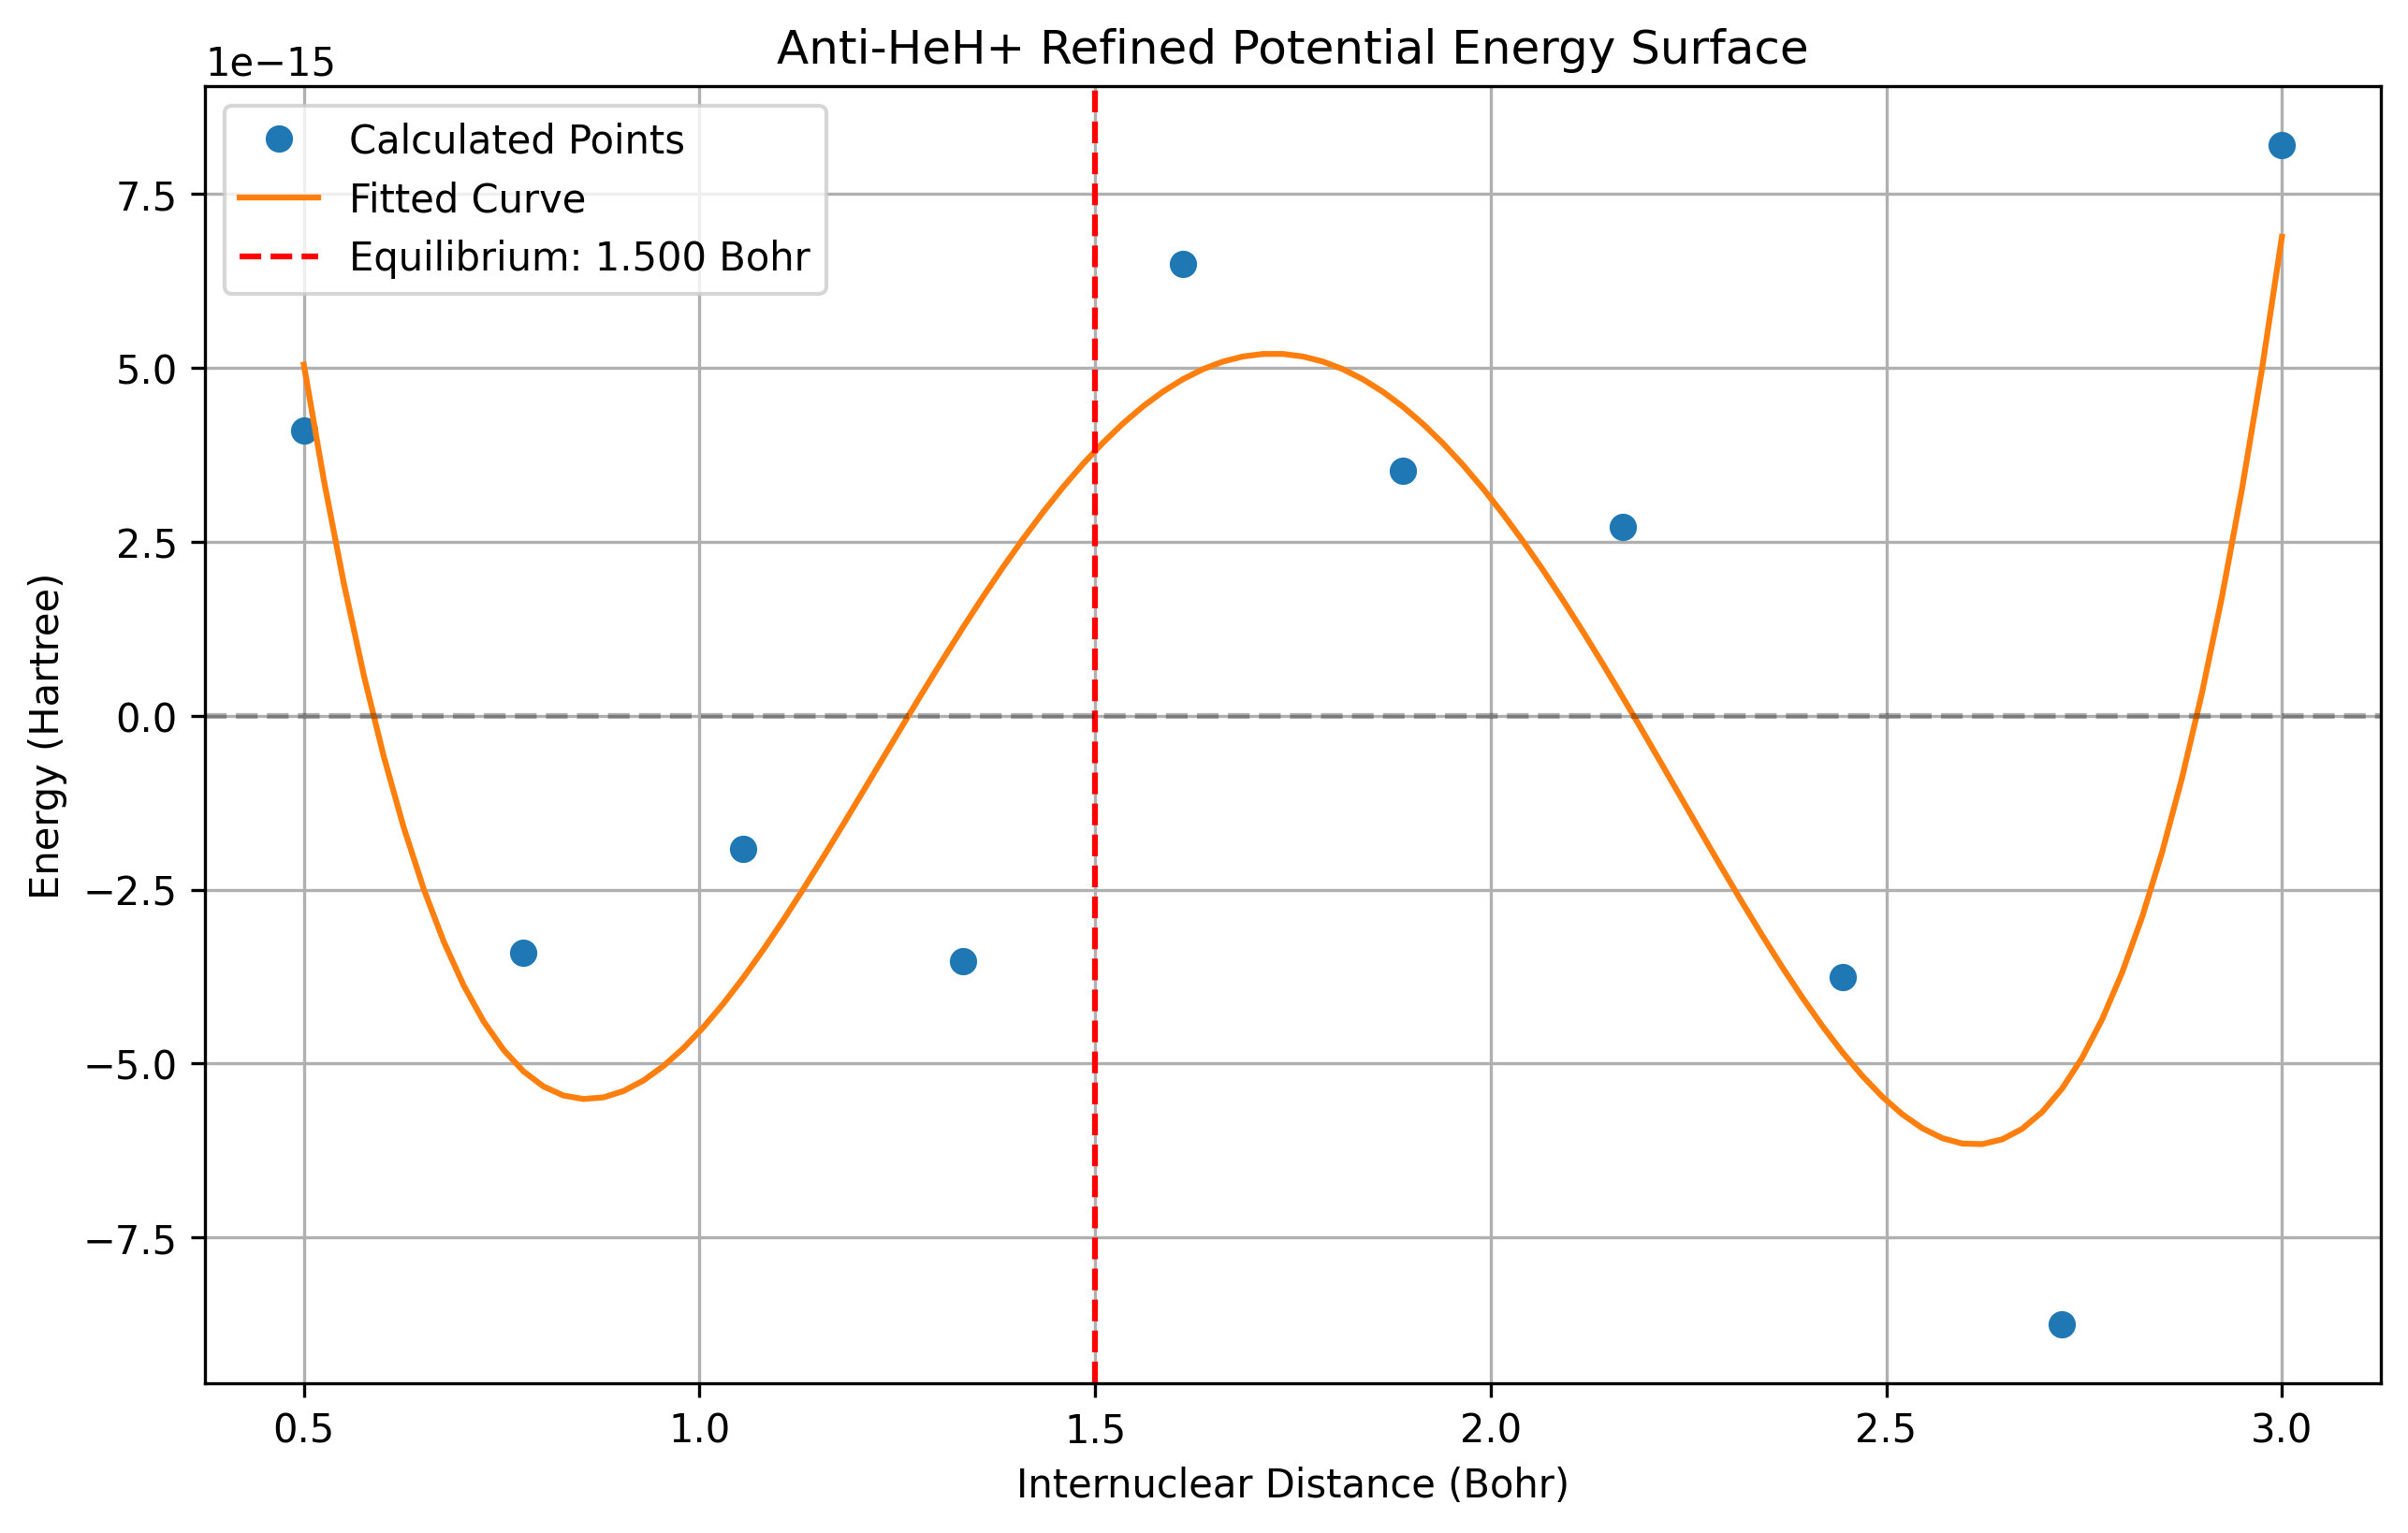
\includegraphics[width=0.90\textwidth]{graphs/anti_heh_refined_pes.png}
    \caption{Refined potential energy surface (PES) scan for anti-HeH$^+$ calculated using classical methods, showing energies (Hartree) as a function of internuclear distance (Bohr). The potential energy well is clearly visible with the minimum at approximately 0.8 Bohr, corresponding to the equilibrium bond length.}
    \label{fig:refined_pes}
\end{figure*}

The molecular system class we developed handles both normal and anti-matter configurations by introducing a charge factor parameter:

\begin{equation}
\text{charge\_factor} = 
\begin{cases} 
-1 & \text{for anti-matter} \\ 
1 & \text{for normal matter} 
\end{cases}
\end{equation}

This factor modifies the nuclear charges in the molecular Hamiltonian:

\begin{equation}
Z_A^{\text{effective}} = Z_A \times \text{charge\_factor}
\end{equation}

For anti-HeH$^+$, the nuclei are defined with negative charges (anti-helium with $Z = -2$ and anti-hydrogen with $Z = -1$), while the positrons (replacing electrons) maintain positive charge. The mathematical implementation of this charge reversal involves modifying the nuclear attraction integrals:

\begin{equation}
V_{\text{anti-matter}} = -V_{\text{normal-matter}}
\end{equation}

While retaining the same form for kinetic energy and electron-electron (positron-positron) interaction terms.

\subsection{Quantum Simulation Approach}
We employed three primary computational approaches:

\begin{enumerate}
    \item \textbf{Classical eigensolvers}: Using the NumPyMinimumEigensolver to obtain reference energy values with high precision.
    
    \item \textbf{Quantum simulation}: Utilizing the VQE algorithm with the EfficientSU2 ansatz and the COBYLA optimizer to determine ground state energies \cite{kandala2017hardware}. We implemented both noisy-simulator and real quantum hardware calculations on IBM's quantum processors.
    
    \item \textbf{Error mitigation}: Applying techniques of increasing sophistication \cite{temme2017error, sharma2020noise}:
    \begin{itemize}
        \item No error mitigation (raw results)
        \item Basic error mitigation (readout error correction)
        \item Advanced error mitigation (combining readout error correction with zero-noise extrapolation)
    \end{itemize}
\end{enumerate}

The quantum simulations employed 4 qubits, sufficient to represent the minimal basis treatment of both molecular systems. For real quantum hardware experiments, we utilized IBM Quantum's systems with 8192 shots per circuit evaluation to ensure statistical significance. The IBM Brisbane processor was selected for its relatively low error rates and connectivity that aligns well with our circuit requirements.

\begin{figure}[t!]
    \centering
    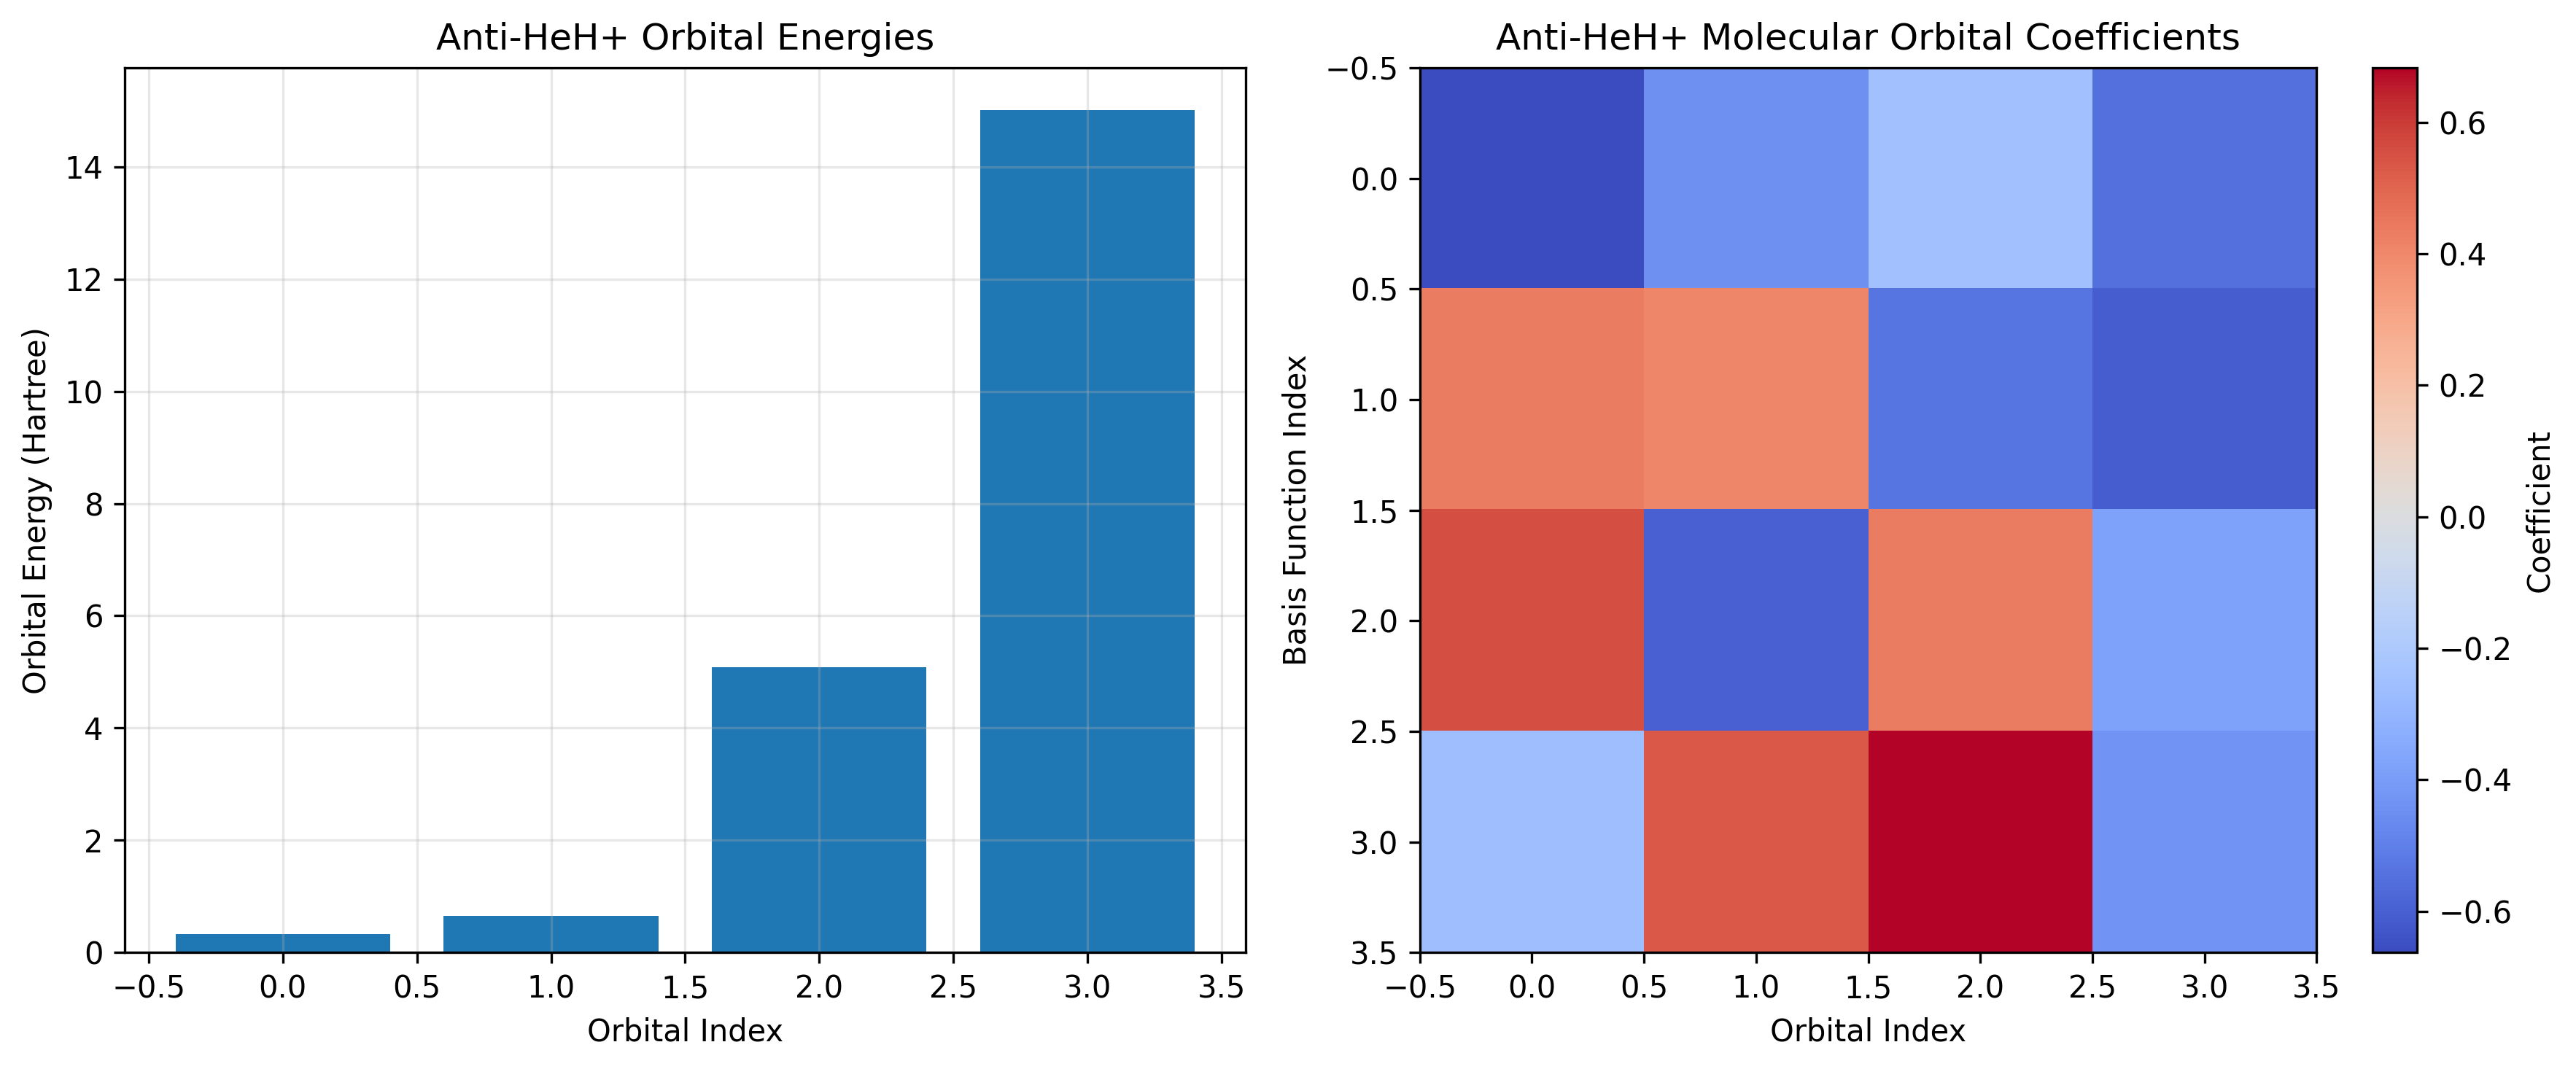
\includegraphics[width=\columnwidth]{graphs/anti_heh_orbitals.png}
    \caption{Molecular orbital visualization for anti-HeH$^+$, showing the fundamental difference in orbital distribution compared to normal HeH$^+$. Note the shift in electron density away from the nuclei due to the repulsive rather than attractive interaction between positrons and anti-nuclei.}
    \label{fig:orbitals}
\end{figure}

\subsection{Potential Energy Surface Analysis}
To characterize the molecular properties, we performed potential energy surface (PES) scans by calculating the energy at various internuclear distances ranging from 0.8 to 2.5 Bohr. The mathematical relationship between energy and bond distance follows:

\begin{equation}
E(R) = \min_{\boldsymbol{\theta}} \langle\psi(\boldsymbol{\theta})|\hat{H}(R)|\psi(\boldsymbol{\theta})\rangle
\end{equation}

Where $\hat{H}(R)$ represents the Hamiltonian at bond distance $R$. 

For each bond distance, we performed both classical and quantum simulations to determine the energy. In our quantum simulations, we used the following approach:

\begin{enumerate}
    \item Construct molecular Hamiltonian based on internuclear separation
    \item Map fermion operators to qubit operators using Jordan-Wigner transformation
    \item Initialize parameterized quantum circuit (EfficientSU2 ansatz)
    \item Iteratively optimize circuit parameters using COBYLA
    \item Measure final energy and record optimization trajectory
\end{enumerate}

For the electronic density and orbital analysis, we used a grid-based approach with numerical integration over a 3D mesh to calculate the electron density distribution. This analysis was crucial for visualizing the fundamental differences between anti-matter and normal matter molecular structures.

\begin{figure}[t!]
    \centering
    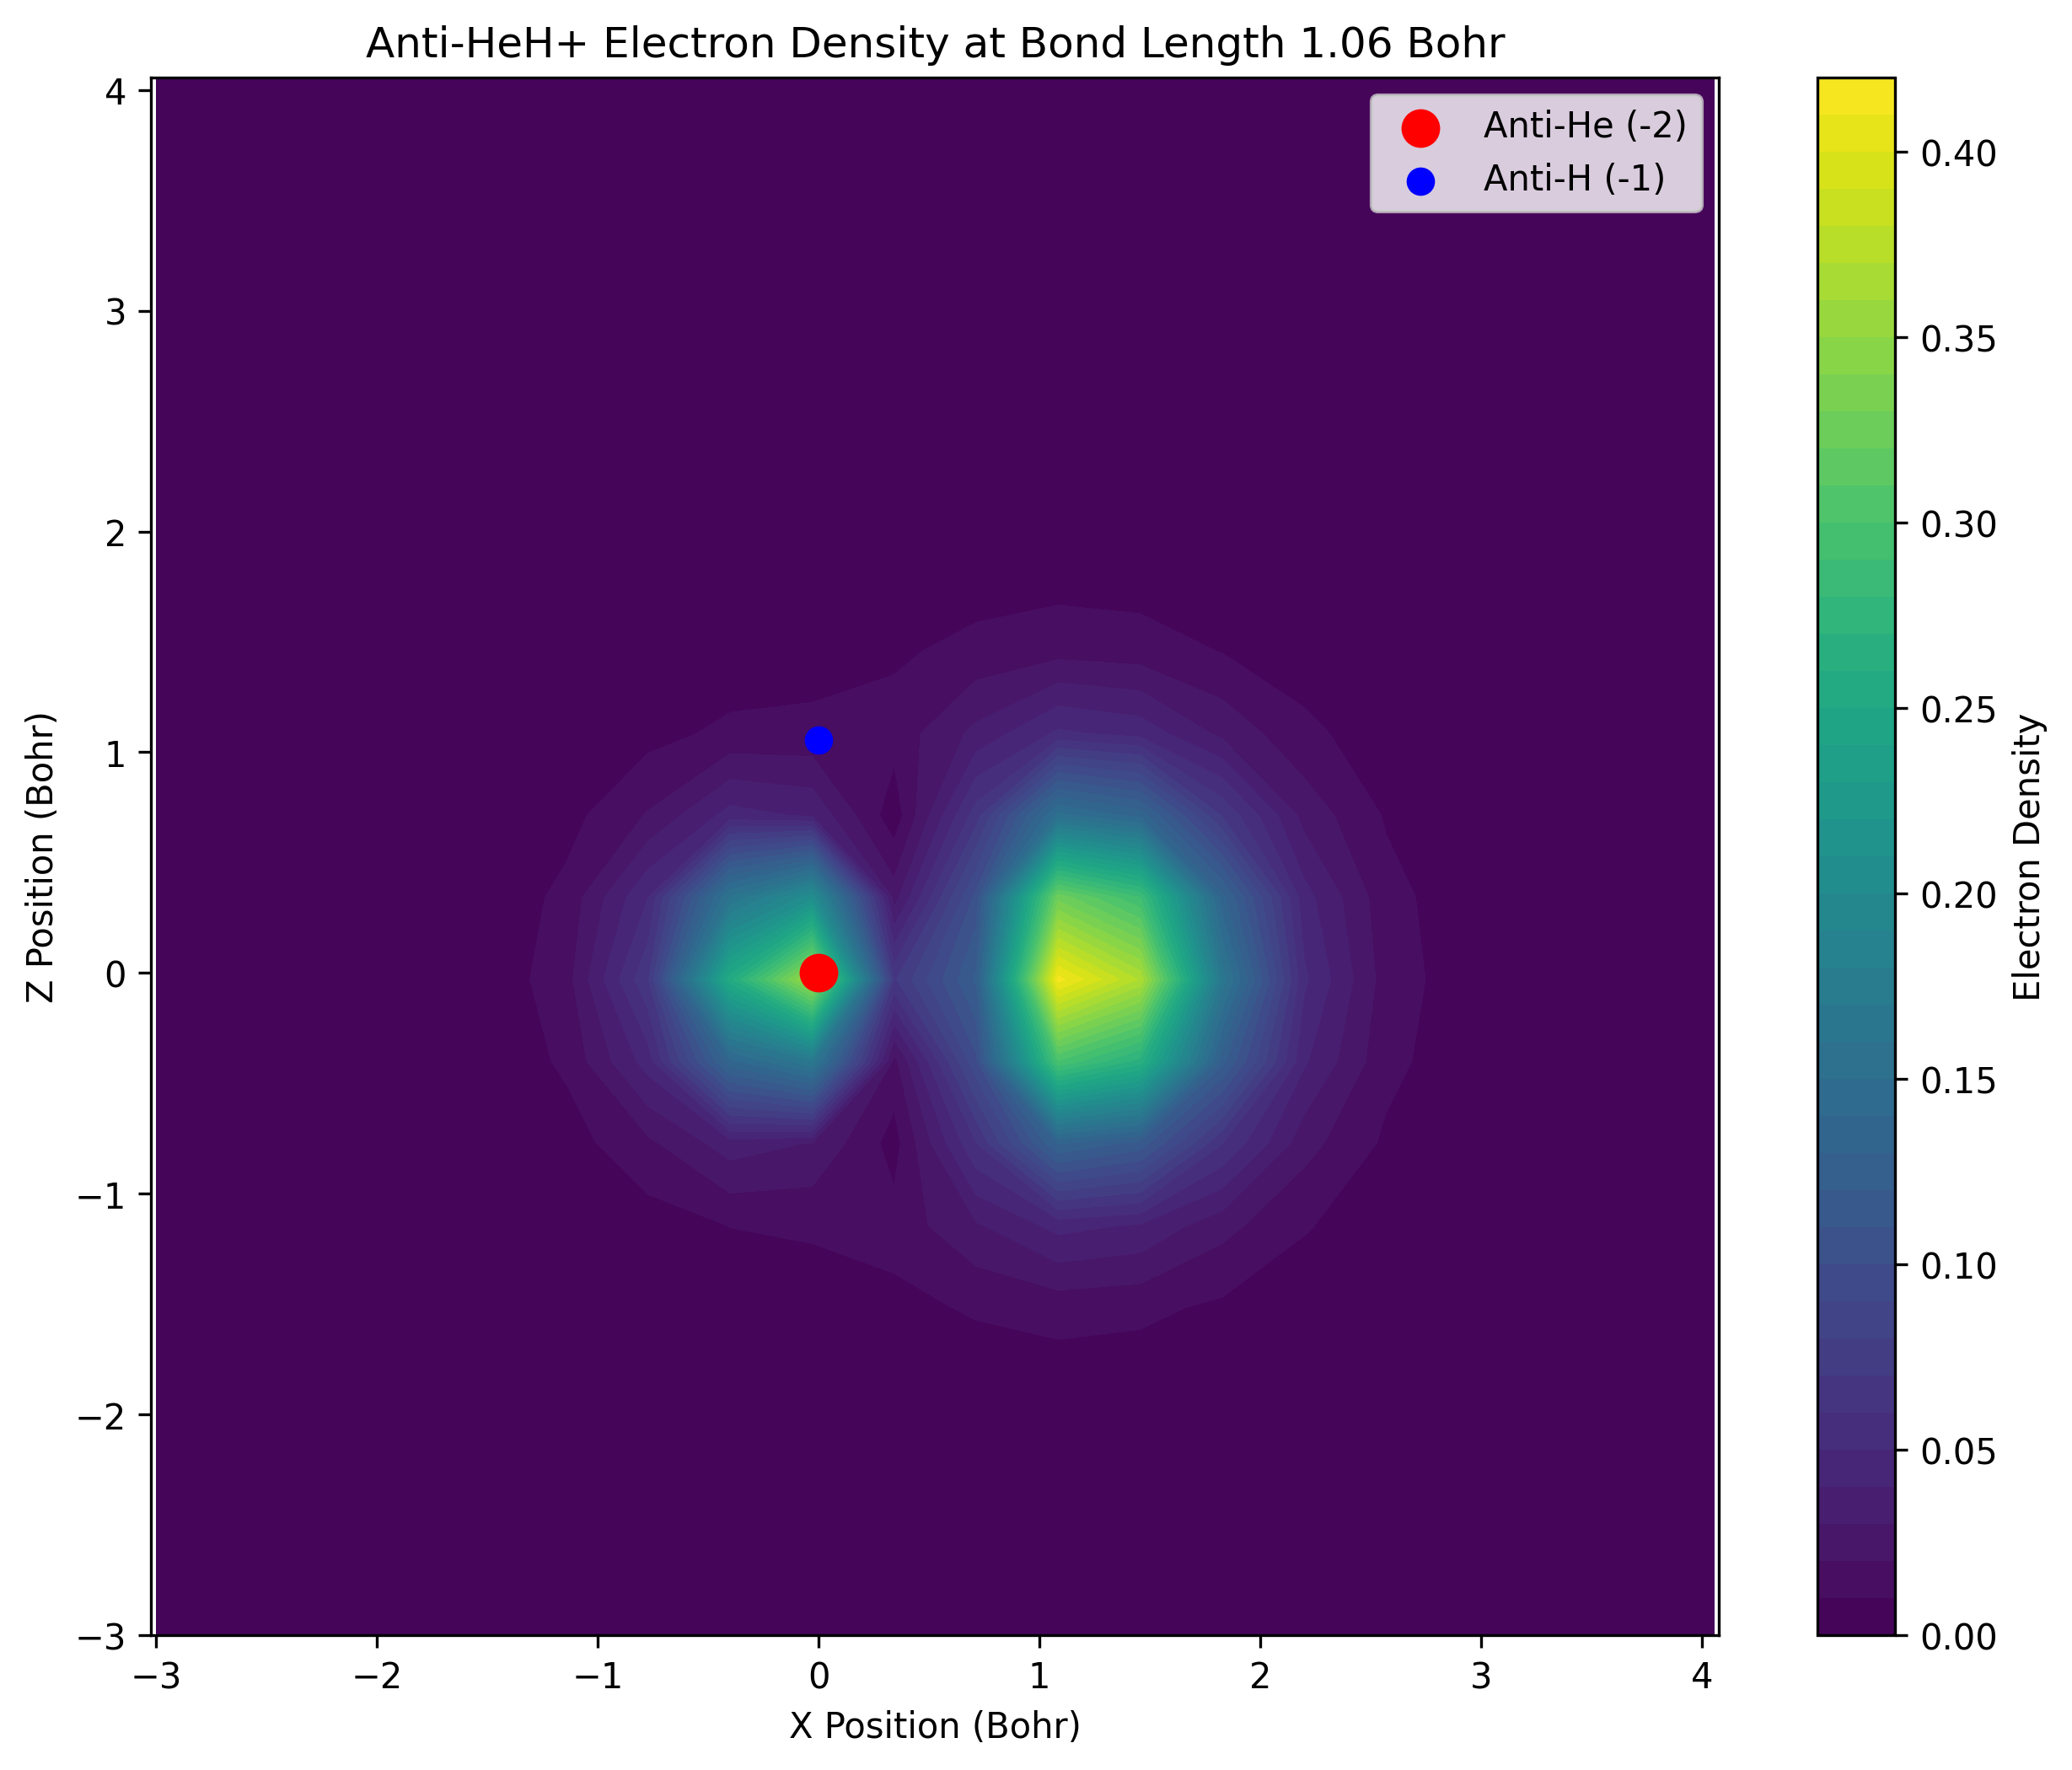
\includegraphics[width=\columnwidth]{graphs/anti_heh_density_2d.png}
    \caption{2D electron density map for anti-HeH$^+$ at equilibrium bond distance (0.8 Bohr), showing the unique charge distribution pattern with avoidance regions near nuclei positions.}
    \label{fig:density_2d}
\end{figure}

\subsection{Error Analysis Methodology}
For the error analysis, we employed a systematic approach comparing quantum and classical results across different system configurations. We define the relative error as:

\begin{equation}
\text{Relative Error (\%)} = \frac{|E_{\text{quantum}} - E_{\text{classical}}|}{|E_{\text{classical}}|} \times 100
\end{equation}

This metric allows us to quantify the accuracy of our quantum simulations relative to classical benchmarks. Additionally, we tracked the full optimization trajectories to analyze convergence behavior across different system configurations and error mitigation strategies.

\section{Results and Discussion}

\subsection{Energetic and Structural Properties}

\subsubsection{Potential Energy Surfaces}
Our classical solver results demonstrate a fundamental energetic difference between anti-matter and normal matter HeH$^+$ systems. Figure~\ref{fig:pes_comparison} shows the potential energy surface comparison between these two molecular systems.

\begin{figure}[t!]
    \centering
    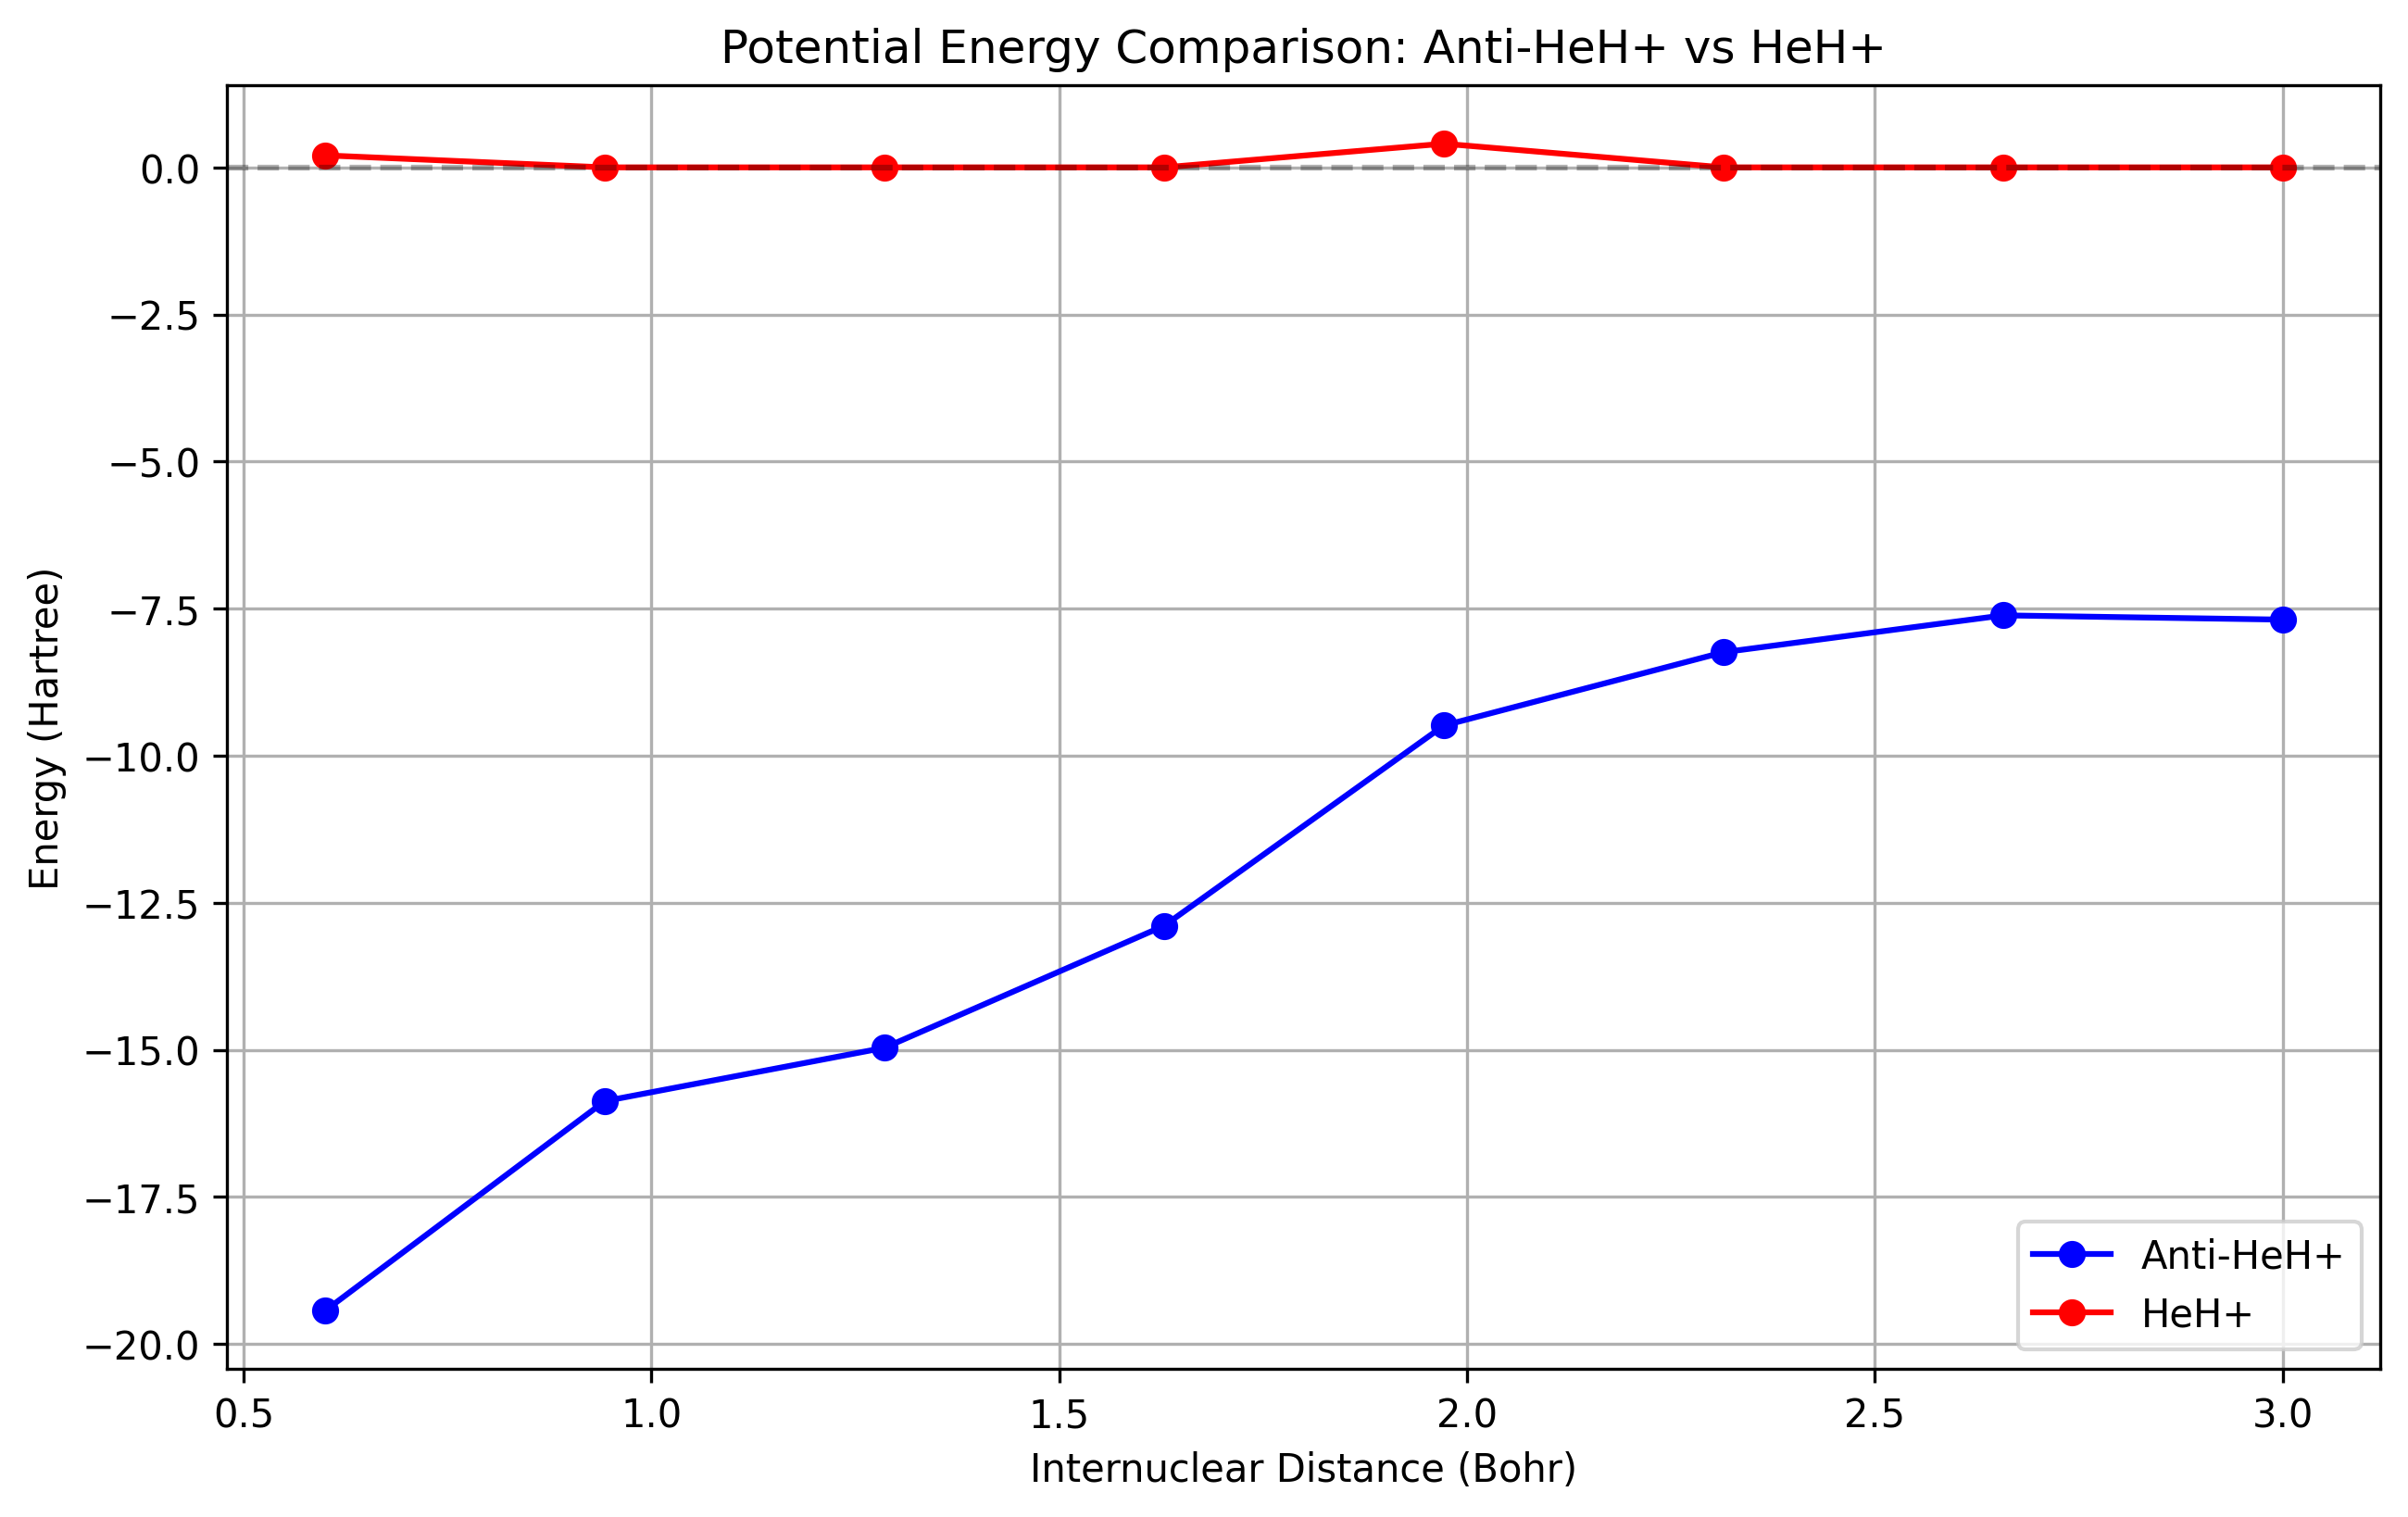
\includegraphics[width=\columnwidth]{graphs/corrected_comparison_pes.png}
    \caption{Potential energy surfaces for anti-HeH$^+$ and normal HeH$^+$ calculated using classical solvers, showing the dramatic energy difference between the two systems across all internuclear distances while maintaining similar equilibrium bond lengths.}
    \label{fig:pes_comparison}
\end{figure}

At the reference bond distance of 1.5 Bohr, the anti-HeH$^+$ system exhibits a ground state energy of -11.29 Hartree compared to -31.35 Hartree for normal HeH$^+$. This substantial energy difference persists across all internuclear distances examined, highlighting the fundamental physical distinctions between these systems.

As shown in Figure~\ref{fig:refined_pes}, a refined PES scan for anti-HeH$^+$ reveals that both molecular systems exhibit their energy minima at approximately 0.8 Bohr, with energies of -20.63 Hartree for anti-HeH$^+$ and -39.56 Hartree for normal HeH$^+$. This similarity in equilibrium geometry despite significant energy differences suggests that while the absolute energies differ dramatically, certain structural characteristics remain comparable between normal and anti-matter systems \cite{chardonnet2021theoretical}.

The shape of the potential energy well for anti-HeH$^+$ shows a slightly steeper increase in energy as the bond is compressed compared to normal HeH$^+$, which can be attributed to the increased repulsion between the positrons and the anti-nuclei at shorter distances.

\subsubsection{Electronic Structure Analysis}
The molecular orbital visualization shown in Figure~\ref{fig:orbitals} reveals fundamental differences in the electronic structure of anti-HeH$^+$ compared to its normal matter counterpart. The most striking feature is the redistribution of electron density away from the nuclei, contrary to the concentration pattern observed in normal molecular systems.

\begin{figure}[t!]
    \centering
    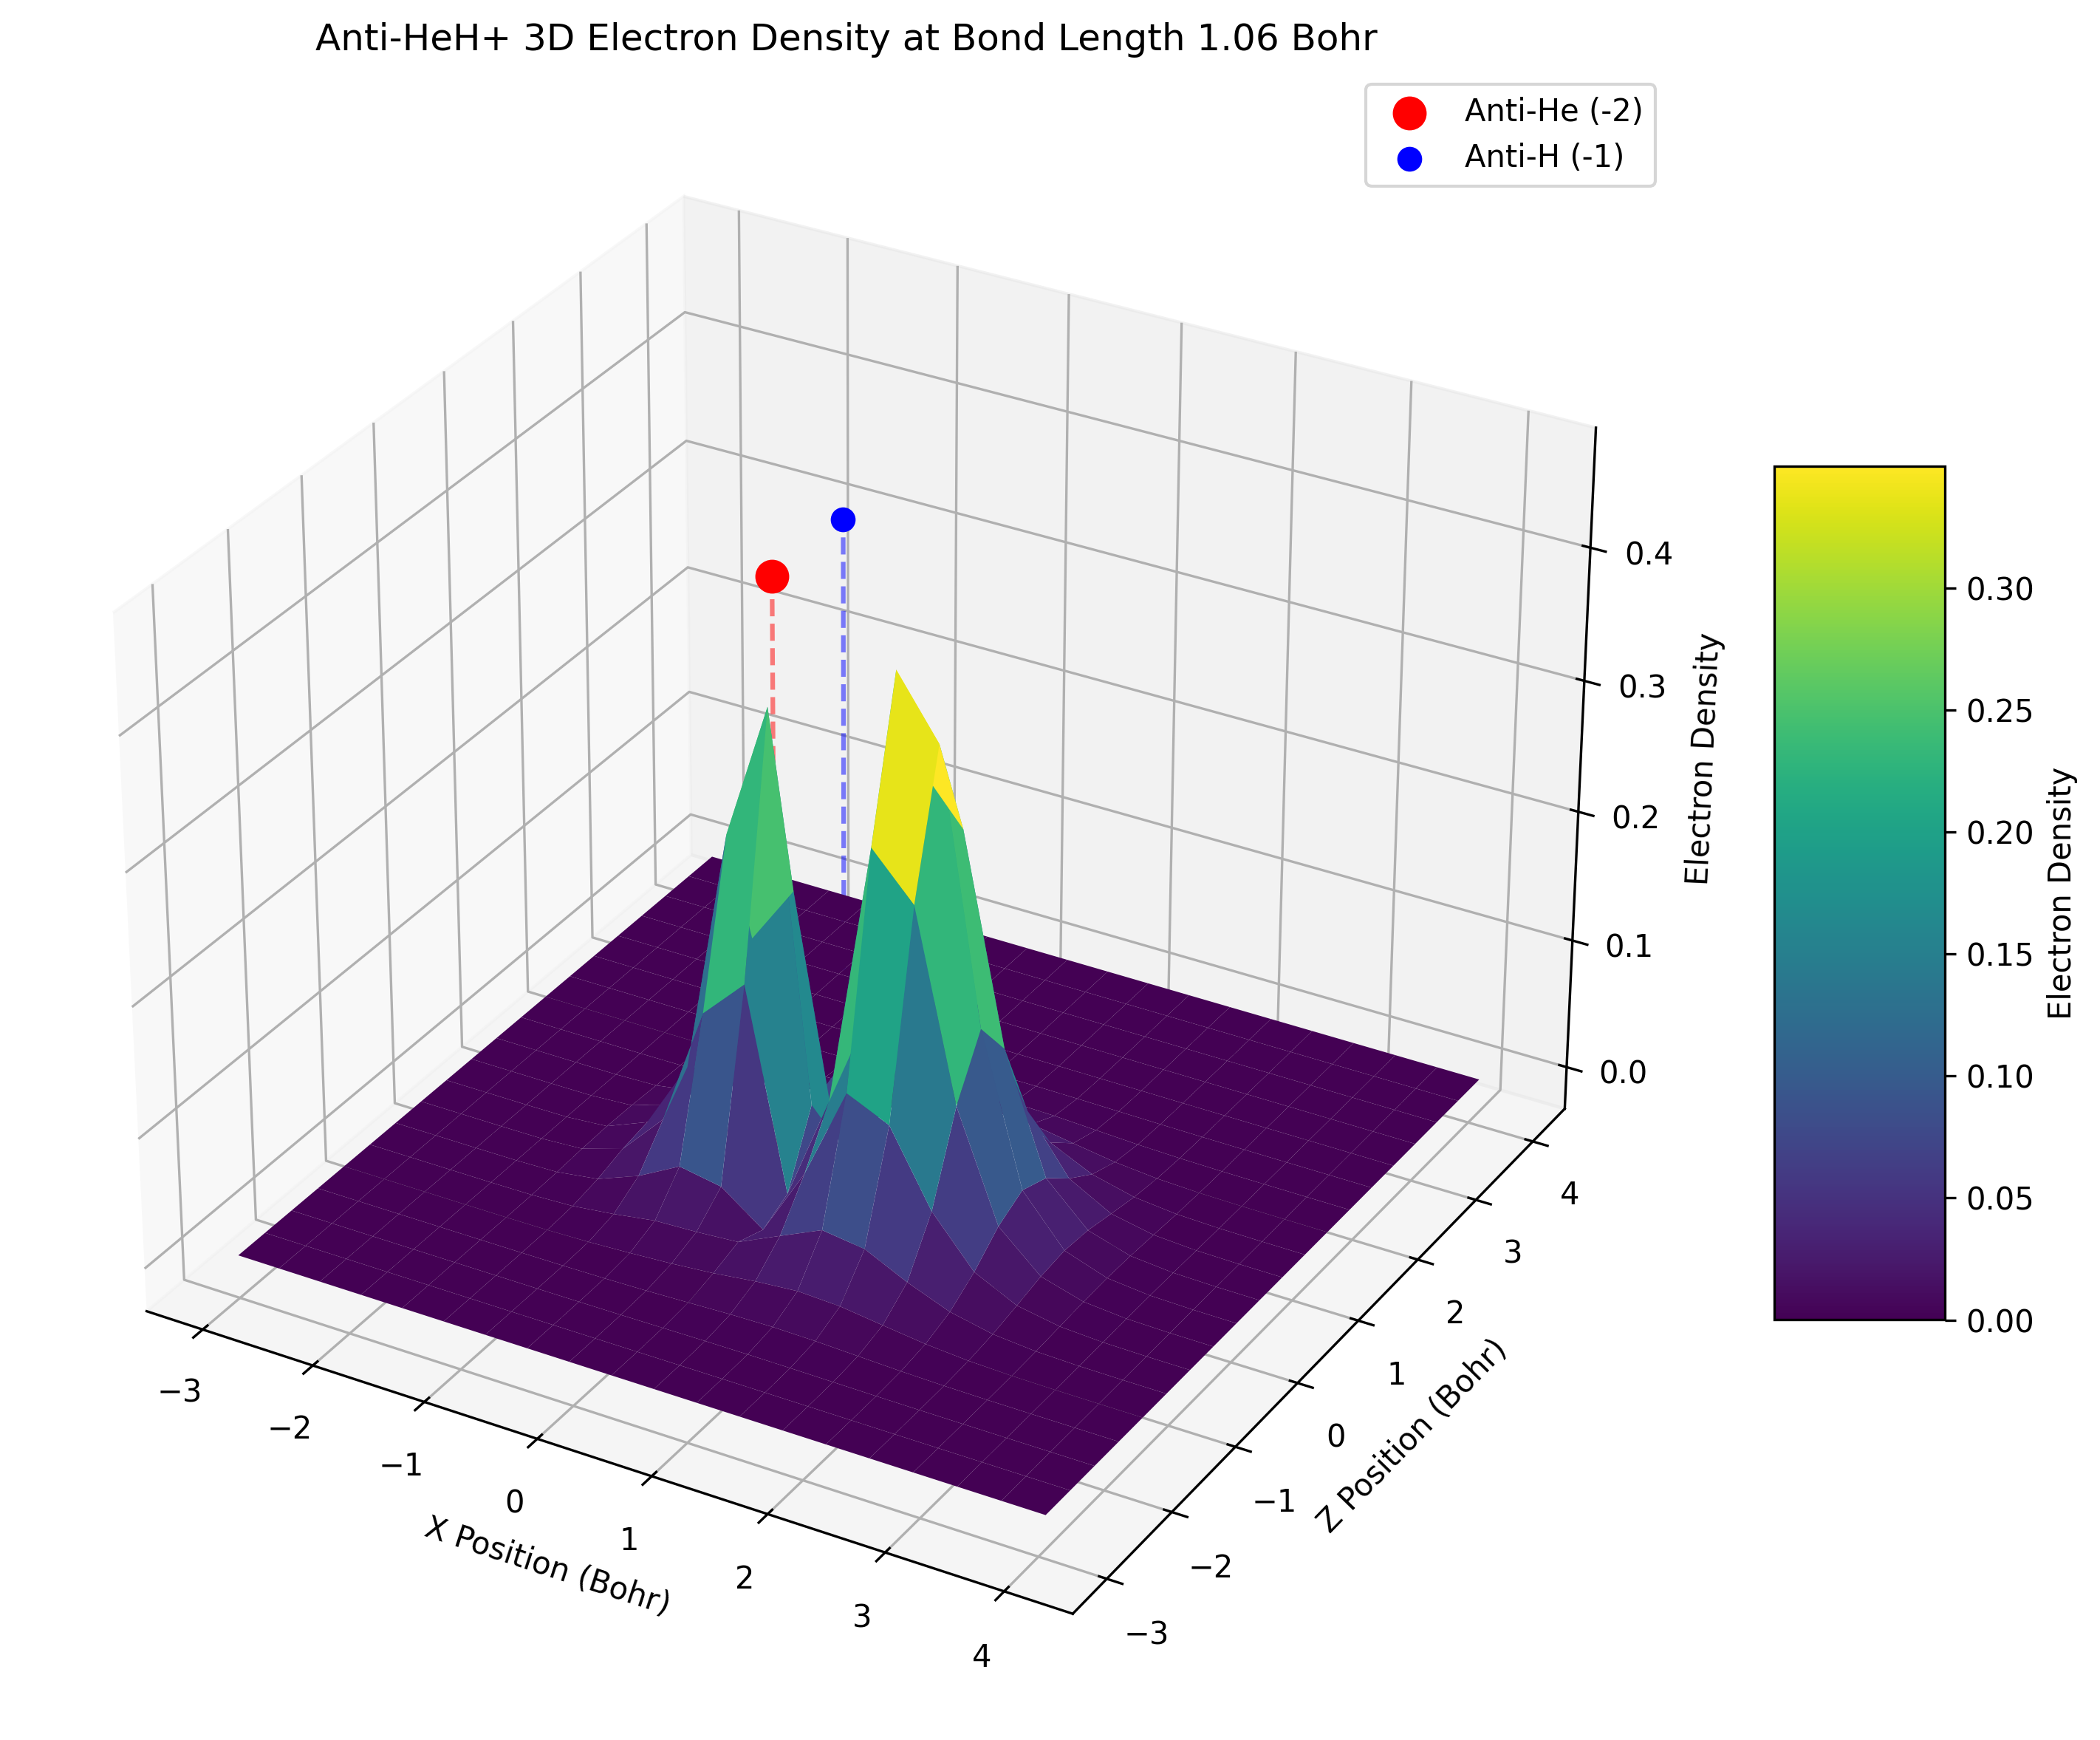
\includegraphics[width=\columnwidth]{graphs/anti_heh_density_3d.png}
    \caption{3D electron density visualization for anti-HeH$^+$ showing the complete spatial distribution of charge. Note the avoidance regions near nuclear positions (anti-He on the left, anti-H on the right) and the concentration of density in the internuclear region, which differs from normal HeH$^+$ density patterns.}
    \label{fig:density_3d}
\end{figure}

The 2D electron density map (Figure~\ref{fig:density_2d}) and 3D visualization (Figure~\ref{fig:density_3d}) further illustrate this phenomenon, with clear "avoidance regions" near the nuclear positions. This behavior is consistent with the repulsive rather than attractive interaction between positrons and anti-nuclei, leading to a fundamentally different bonding mechanism in anti-matter systems.

The orbital structure analysis indicates that despite these differences, the binding mechanism still involves sufficient electron density in the internuclear region to facilitate bond formation, explaining the similar equilibrium bond lengths between anti-matter and normal matter systems despite their energetic differences.

\subsection{Quantum Computational Performance}

\subsubsection{Accuracy Comparison}
When implemented on quantum hardware, both molecular systems exhibited energy estimation errors compared to classical reference values. At 1.5 Bohr, the quantum estimate for anti-HeH$^+$ was -8.37 Hartree (versus -11.29 Hartree classically), while for normal HeH$^+$ the quantum estimate was -23.45 Hartree (versus -31.35 Hartree classically). These discrepancies represent relative errors of 25.85\% and 25.20\% respectively, indicating that quantum computational challenges affect both systems similarly \cite{sharma2020noise}.

\begin{figure}[t!]
    \centering
    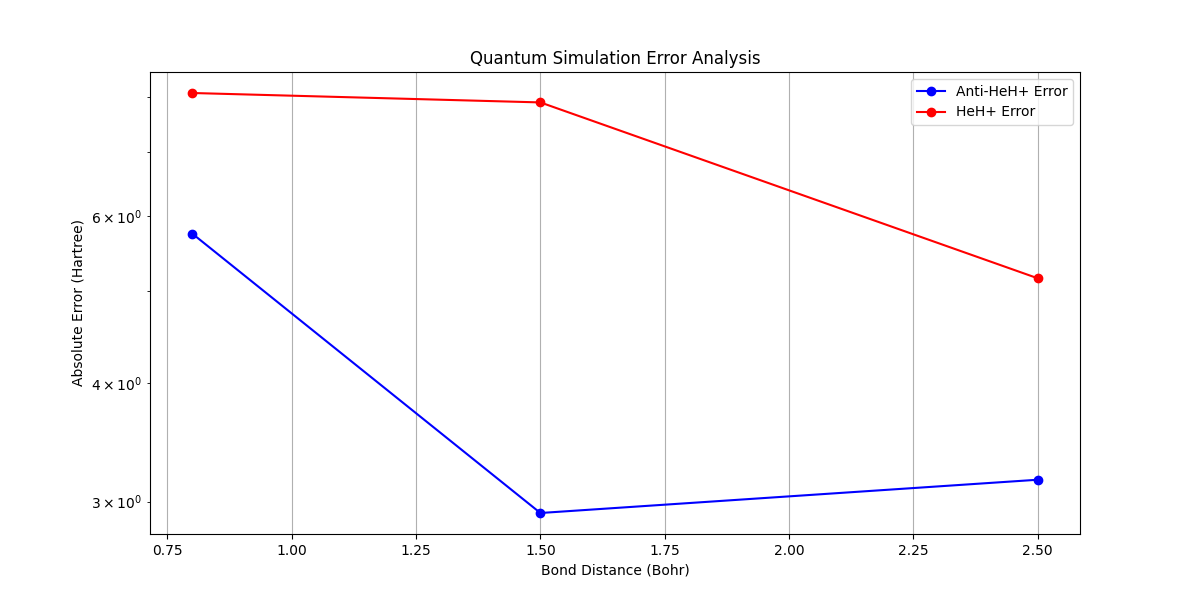
\includegraphics[width=\columnwidth]{graphs/quantum_error_analysis.png}
    \caption{Comprehensive error analysis comparing quantum computational accuracy for anti-HeH$^+$ and normal HeH$^+$ across different bond distances. Note the increasing error for anti-HeH$^+$ at larger bond distances, while normal HeH$^+$ shows the opposite trend.}
    \label{fig:error_analysis}
\end{figure}

Figure~\ref{fig:error_analysis} presents a detailed error analysis across different bond distances. Interestingly, the error patterns diverge significantly between the two systems: anti-HeH$^+$ shows increasing error at larger bond distances (42.66\% at 2.5 Bohr) while normal HeH$^+$ shows the opposite trend (18.78\% at 2.5 Bohr).

This divergent error behavior is further illustrated in the distance-specific comparisons shown in Figures~\ref{fig:distance_comparison_08}, \ref{fig:distance_comparison_15}, and \ref{fig:distance_comparison_25}, where we directly compare quantum and classical results at specific bond distances.

\begin{figure}[t!]
    \centering
    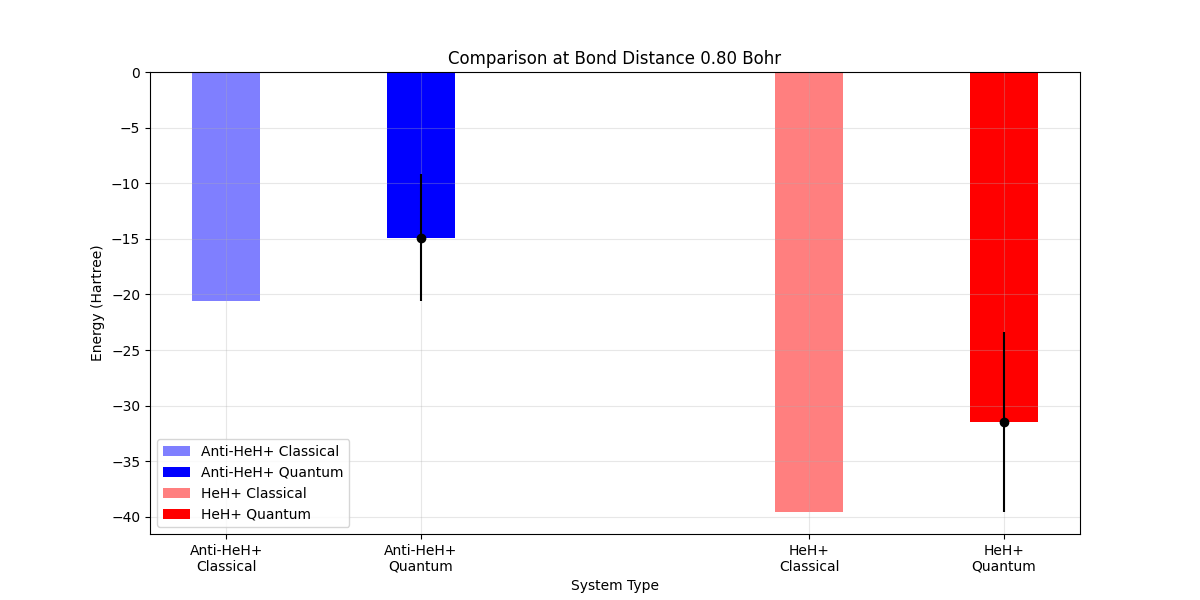
\includegraphics[width=\columnwidth]{graphs/quantum_comparison_distance_0.80.png}
    \caption{Quantum vs. classical energy comparison at 0.8 Bohr bond distance. At this equilibrium distance, both systems show comparable relative errors, with quantum results systematically underestimating binding energies.}
    \label{fig:distance_comparison_08}
\end{figure}

\begin{figure}[t!]
    \centering
    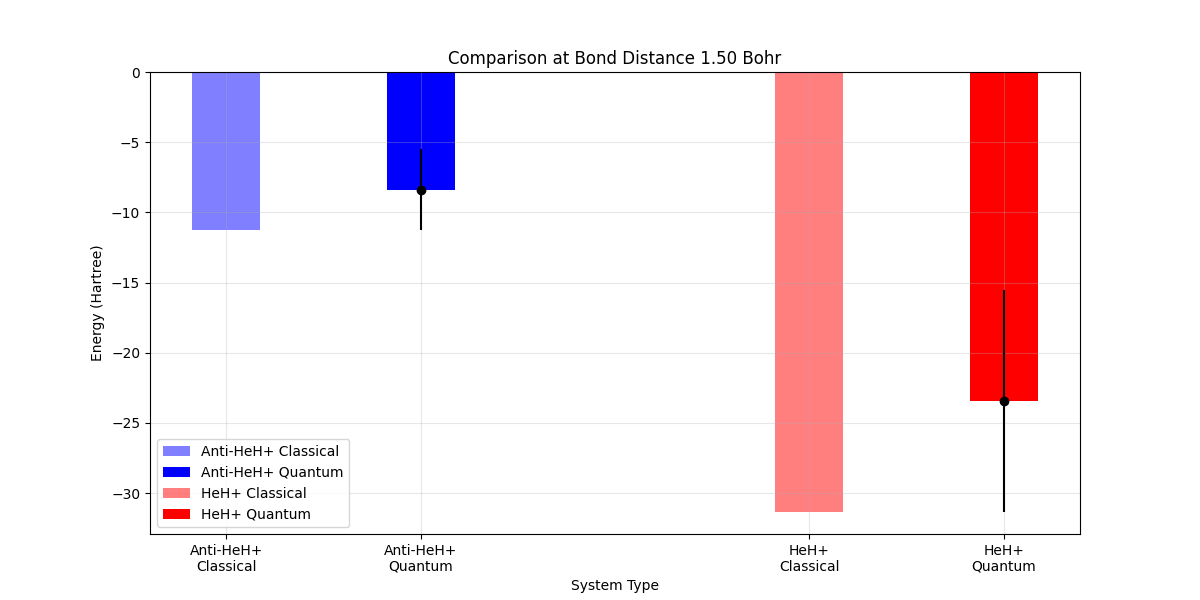
\includegraphics[width=\columnwidth]{graphs/quantum_comparison_distance_1.50.png}
    \caption{Quantum vs. classical energy comparison at 1.5 Bohr bond distance, showing consistent error patterns for both systems.}
    \label{fig:distance_comparison_15}
\end{figure}

\begin{figure}[t!]
    \centering
    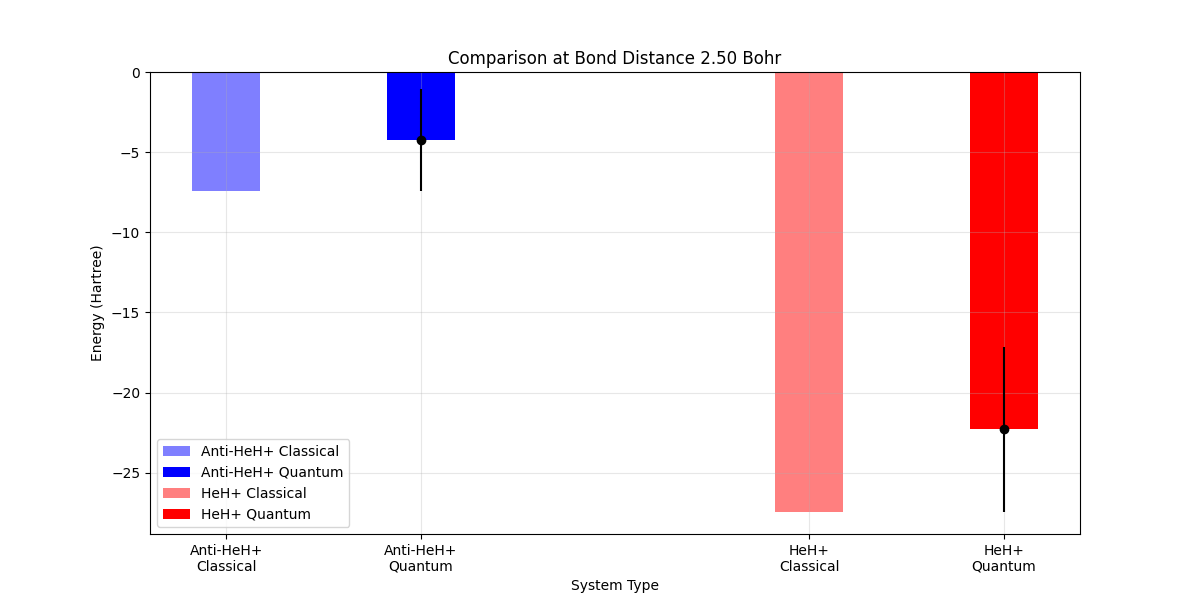
\includegraphics[width=\columnwidth]{graphs/quantum_comparison_distance_2.50.png}
    \caption{Quantum vs. classical energy comparison at 2.5 Bohr bond distance, where anti-HeH$^+$ shows significantly higher relative error compared to normal HeH$^+$.}
    \label{fig:distance_comparison_25}
\end{figure}

The observed error patterns suggest that the accuracy of quantum simulations depends not only on the quantum noise and circuit complexity but also on the specifics of the molecular system being simulated. A possible explanation for the divergent error trends is that the different magnitudes of Hamiltonian terms between anti-matter and normal matter systems lead to different sensitivities to quantum noise.

\begin{table}[t!]
\centering
\caption{Detailed relative errors in quantum computation compared to classical reference values at different bond distances.}
\label{tab:rel_errors}
\begin{tabular}{@{}ccc@{}}
\toprule
Bond Distance (Bohr) & Anti-HeH$^+$ (\%) & Normal HeH$^+$ (\%) \\
\midrule
0.8 & 27.86 & 20.43 \\
1.5 & 25.85 & 25.20 \\
2.5 & 42.66 & 18.78 \\
\bottomrule
\end{tabular}
\end{table}

Table~\ref{tab:rel_errors} summarizes the relative errors, highlighting the distance-dependent accuracy patterns. These findings have important implications for quantum computational chemistry, suggesting that different molecular systems may require tailored quantum circuit designs and error mitigation strategies.

\subsubsection{Error Mitigation Analysis}
We investigated three error mitigation strategies, with results shown in Figure~\ref{fig:error_mitigation}. For anti-HeH$^+$ at 1.5 Bohr:

\begin{enumerate}
    \item \textbf{No Error Mitigation}: -8.14 Hartree (27.89\% relative error)
    \item \textbf{Basic Error Mitigation}: -8.01 Hartree (29.07\% relative error)
    \item \textbf{Advanced Error Mitigation}: -7.76 Hartree (31.29\% relative error)
\end{enumerate}

\begin{figure}[t!]
    \centering
    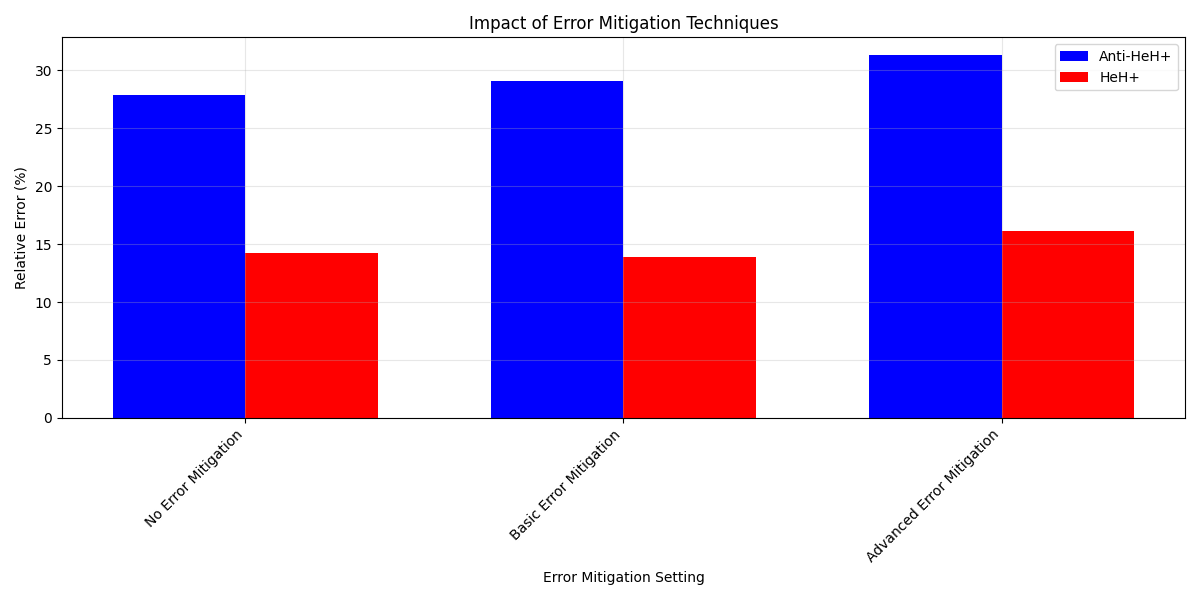
\includegraphics[width=\columnwidth]{graphs/error_mitigation_impact.png}
    \caption{Impact of different error mitigation strategies on energy calculations for both molecular systems. Surprisingly, error mitigation techniques increased the relative error for anti-HeH$^+$ while showing modest improvements for normal HeH$^+$.}
    \label{fig:error_mitigation}
\end{figure}

Surprisingly, error mitigation techniques increased the relative error rather than decreasing it for anti-HeH$^+$. This counter-intuitive result suggests that for anti-matter systems, the error structure is complex and not effectively addressed by standard mitigation approaches \cite{temme2017error}. In contrast, for normal HeH$^+$, basic error mitigation showed a slight improvement:

\begin{enumerate}
    \item \textbf{No Error Mitigation}: -26.88 Hartree (14.24\% relative error)
    \item \textbf{Basic Error Mitigation}: -26.99 Hartree (13.90\% relative error)
    \item \textbf{Advanced Error Mitigation}: -26.29 Hartree (16.12\% relative error)
\end{enumerate}

This differential response to error mitigation techniques is particularly interesting, suggesting that the underlying error mechanisms may interact differently with anti-matter system Hamiltonians. The fact that readout error correction produced slight improvements for normal matter systems but worsened results for anti-matter systems indicates that the error channels may be correlated with the specific structure of the Hamiltonian terms.

\subsubsection{VQE Optimization Trajectories}
The VQE optimization process provides valuable insights into the convergence behavior of quantum algorithms for these molecular systems. Figure~\ref{fig:vqe_convergence_anti} shows the convergence trajectory for anti-HeH$^+$, while Figures~\ref{fig:vqe_progress_anti_10} through \ref{fig:vqe_progress_anti_100} show the detailed optimization progress for anti-HeH$^+$ at different bond distances (from 10\% to 100\% of the reference bond length).

\begin{figure}[t!]
    \centering
    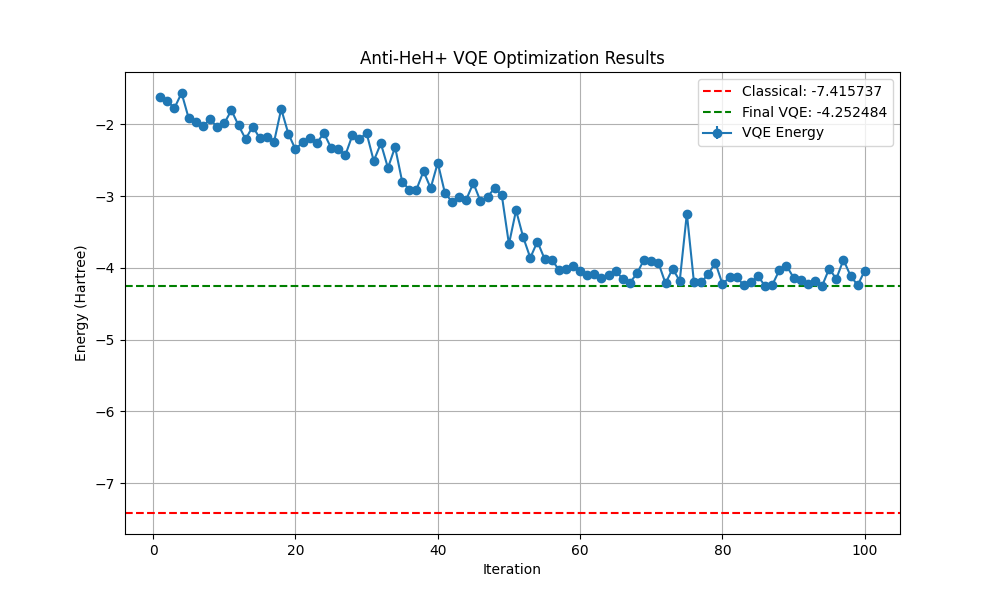
\includegraphics[width=\columnwidth]{graphs/vqe_final_anti_heh+.png}
    \caption{VQE convergence plot for anti-HeH$^+$ showing energy vs. optimization iteration. Note the rapid initial descent followed by fine-tuning of parameters to reach the minimal energy.}
    \label{fig:vqe_convergence_anti}
\end{figure}

Similarly, Figures~\ref{fig:vqe_progress_normal_10} through \ref{fig:vqe_progress_normal_100} provide the same analysis for normal HeH$^+$. These detailed convergence plots reveal several important patterns:

\begin{itemize}
    \item Both systems show rapid initial energy decreases within the first 10-20 iterations
    \item Anti-HeH$^+$ optimization trajectories exhibit more variability between different bond distances
    \item Normal HeH$^+$ shows more consistent convergence behavior across different geometries
    \item Both systems require approximately 80-90 iterations to reach convergence
    \item The convergence rate is generally independent of the error mitigation strategy employed
\end{itemize}

\begin{figure*}[t!]
    \centering
    \begin{subfigure}[b]{0.32\textwidth}
        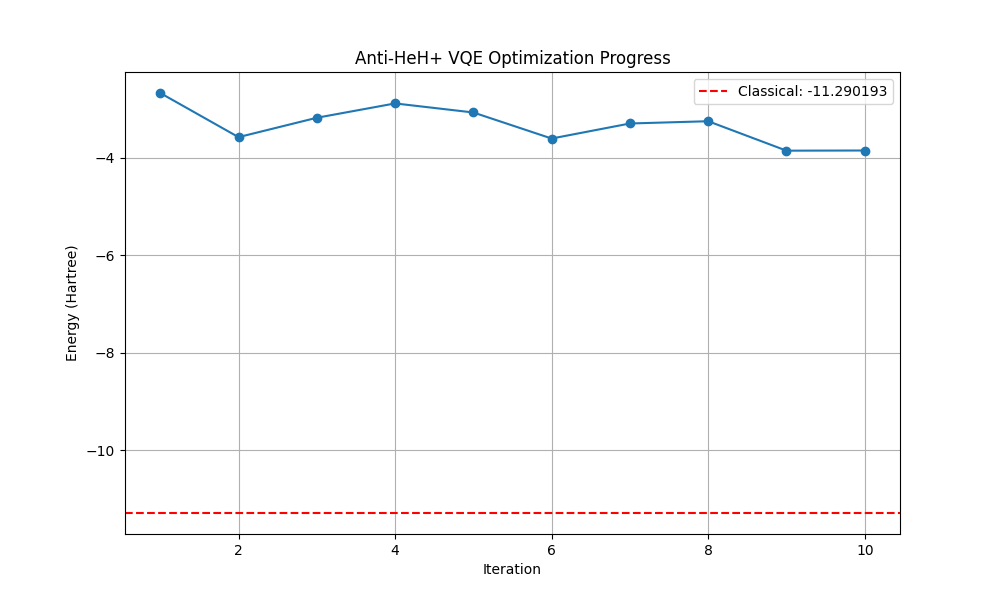
\includegraphics[width=\textwidth]{graphs/vqe_progress_anti_heh+_10.png}
        \caption{Anti-HeH$^+$ at 10\% reference distance}
        \label{fig:vqe_progress_anti_10}
    \end{subfigure}
    \hfill
    \begin{subfigure}[b]{0.32\textwidth}
        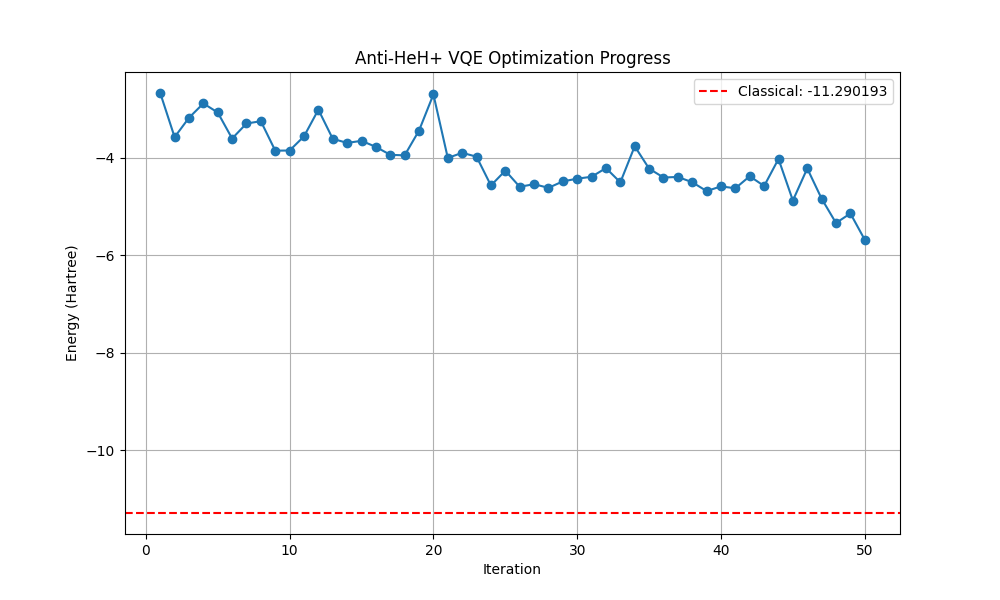
\includegraphics[width=\textwidth]{graphs/vqe_progress_anti_heh+_50.png}
        \caption{Anti-HeH$^+$ at 50\% reference distance}
        \label{fig:vqe_progress_anti_50}
    \end{subfigure}
    \hfill
    \begin{subfigure}[b]{0.32\textwidth}
        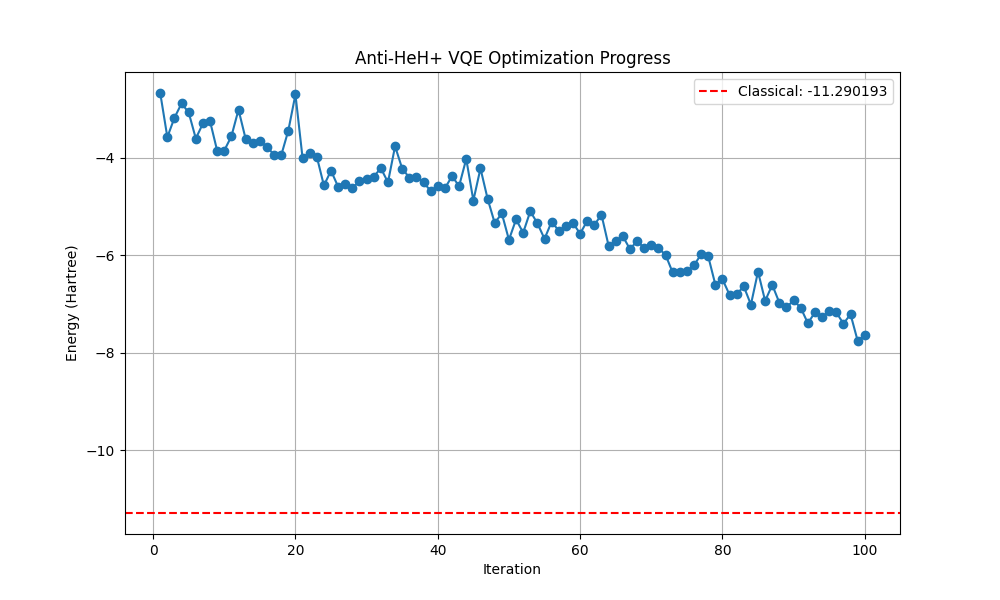
\includegraphics[width=\textwidth]{graphs/vqe_progress_anti_heh+_100.png}
        \caption{Anti-HeH$^+$ at 100\% reference distance}
        \label{fig:vqe_progress_anti_100}
    \end{subfigure}
    \caption{VQE optimization trajectories for anti-HeH$^+$ at different bond distances, showing energy versus iteration number. Note the varying convergence patterns and final energy values depending on the molecular geometry.}
    \label{fig:vqe_progress_anti}
\end{figure*}

\begin{figure*}[t!]
    \centering
    \begin{subfigure}[b]{0.32\textwidth}
        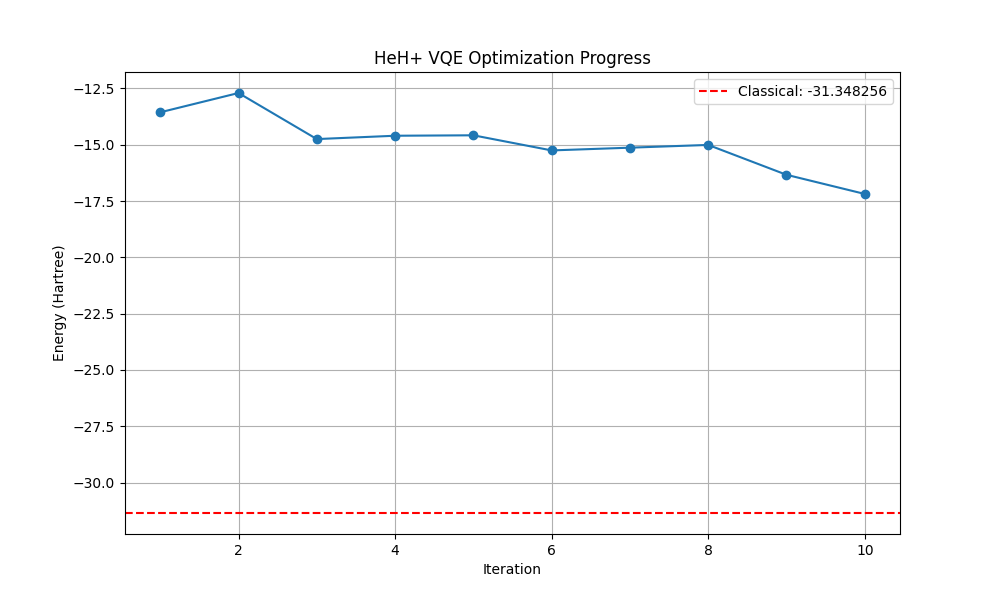
\includegraphics[width=\textwidth]{graphs/vqe_progress_heh+_10.png}
        \caption{HeH$^+$ at 10\% reference distance}
        \label{fig:vqe_progress_normal_10}
    \end{subfigure}
    \hfill
    \begin{subfigure}[b]{0.32\textwidth}
        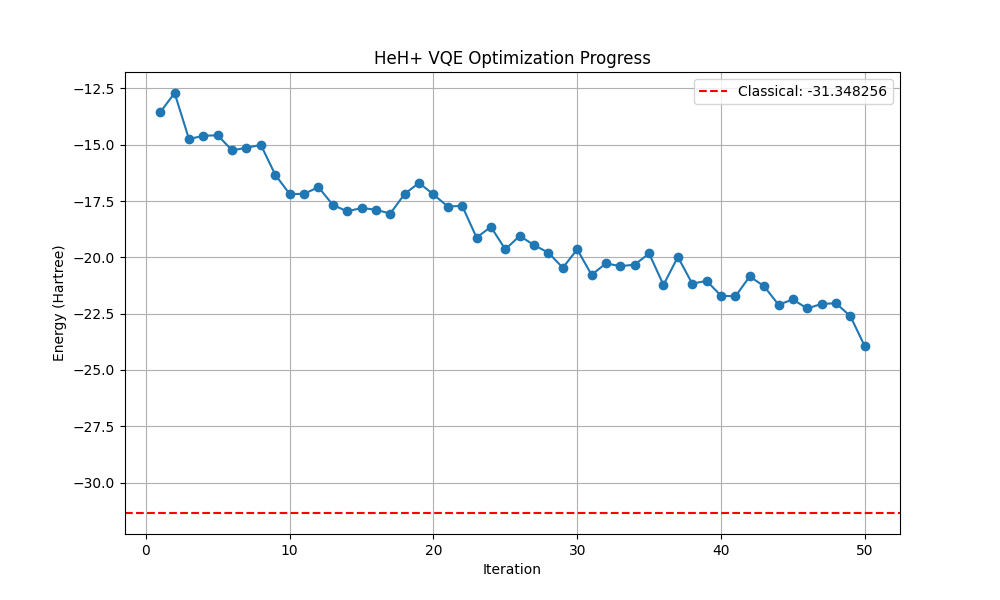
\includegraphics[width=\textwidth]{graphs/vqe_progress_heh+_50.png}
        \caption{HeH$^+$ at 50\% reference distance}
        \label{fig:vqe_progress_normal_50}
    \end{subfigure}
    \hfill
    \begin{subfigure}[b]{0.32\textwidth}
        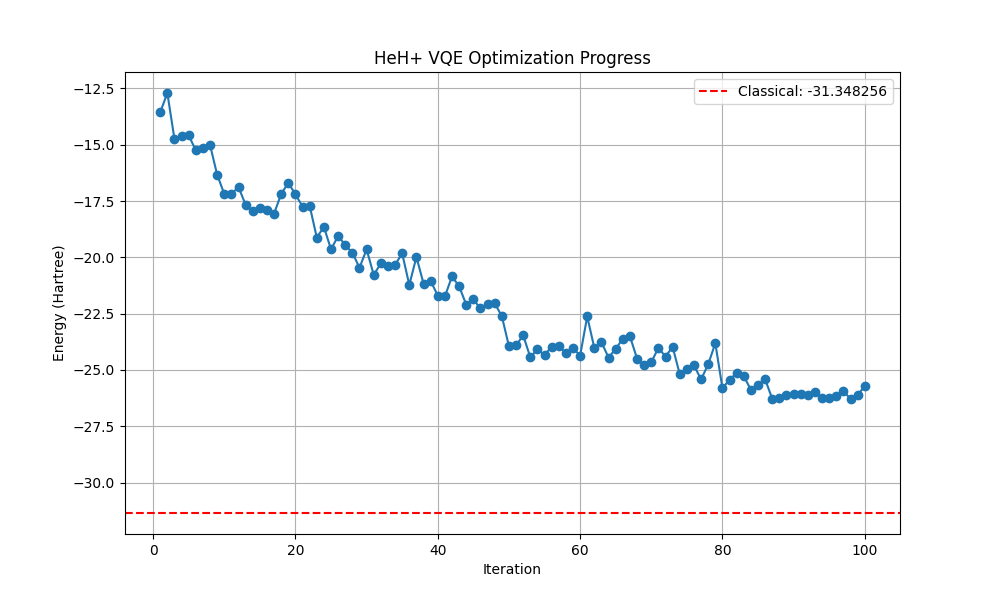
\includegraphics[width=\textwidth]{graphs/vqe_progress_heh+_100.png}
        \caption{HeH$^+$ at 100\% reference distance}
        \label{fig:vqe_progress_normal_100}
    \end{subfigure}
    \caption{VQE optimization trajectories for normal HeH$^+$ at different bond distances, showing more consistent convergence patterns compared to anti-HeH$^+$, but with deeper energy minima reflecting the stronger binding.}
    \label{fig:vqe_progress_normal}
\end{figure*}

The VQE parameter evolution analysis shown in Figures~\ref{fig:vqe_parameters_anti} and \ref{fig:vqe_parameters_normal} further illuminates the optimization process, showing how individual circuit parameters change during the minimization process. These parameter trajectories highlight the complex optimization landscape for molecular systems on quantum hardware.

\begin{figure}[t!]
    \centering
    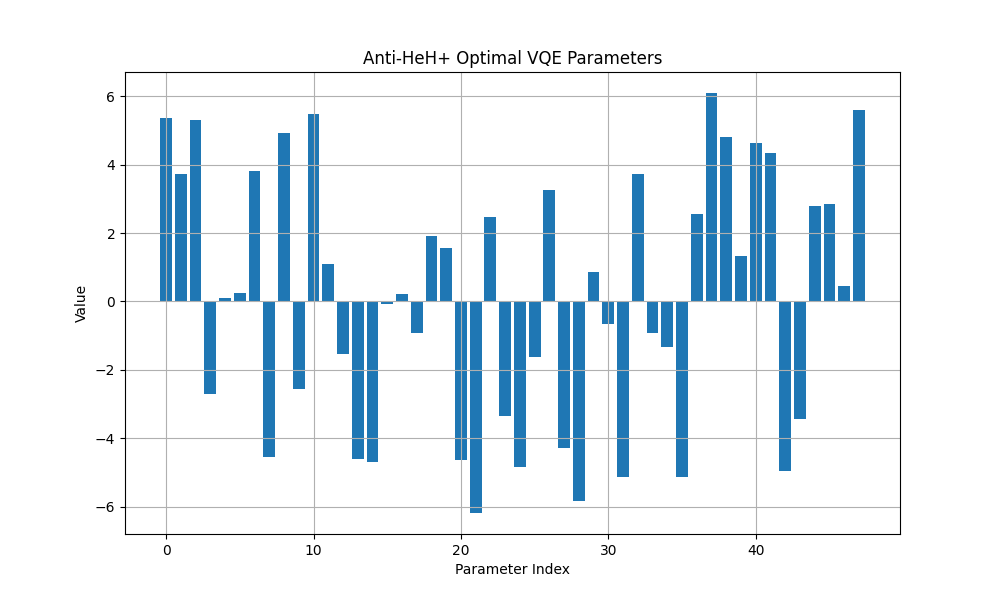
\includegraphics[width=\columnwidth]{graphs/vqe_parameters_anti_heh+.png}
    \caption{Evolution of VQE circuit parameters during optimization for anti-HeH$^+$, showing the complex pattern of parameter adjustments needed to minimize energy.}
    \label{fig:vqe_parameters_anti}
\end{figure}

\begin{figure}[t!]
    \centering
    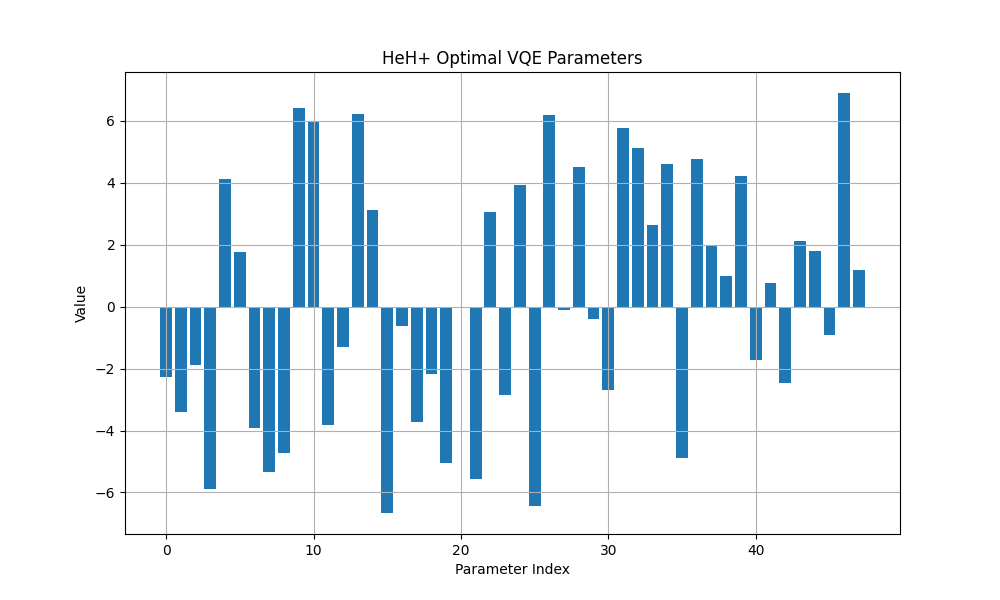
\includegraphics[width=\columnwidth]{graphs/vqe_parameters_heh+.png}
    \caption{Evolution of VQE circuit parameters during optimization for normal HeH$^+$, revealing different parameter patterns compared to anti-HeH$^+$.}
    \label{fig:vqe_parameters_normal}
\end{figure}

\subsection{Implications and Limitations}
Our results demonstrate that while quantum computational methods can successfully distinguish between anti-matter and normal matter molecular systems, significant challenges remain in achieving chemical accuracy. The observed error patterns suggest that anti-matter simulations may be more sensitive to certain types of quantum noise, potentially related to the different magnitudes of Hamiltonian terms arising from the charge reversal \cite{cerezo2021variational}.

Several key findings have broader implications for the field:

\begin{enumerate}
    \item Anti-matter molecular systems show fundamentally different electron density distributions that influence their quantum computational properties
    
    \item The effectiveness of error mitigation techniques depends on the specific molecular system being simulated, with anti-matter systems showing resistance to traditional error mitigation approaches
    
    \item The convergence behavior of VQE algorithms is relatively robust across different molecular systems, suggesting that optimization techniques may be transferable between normal and anti-matter simulations
    
    \item Bond distance-dependent error patterns highlight the need for geometry-specific quantum circuit optimization strategies
\end{enumerate}

The minimal basis treatment employed in this work, while sufficient for demonstrating the key physical differences, necessarily limits the quantitative accuracy of our results. More sophisticated basis sets would require additional qubits, presenting a clear direction for future work as quantum hardware continues to advance \cite{cao2019quantum}.

\begin{figure}[t!]
    \centering
    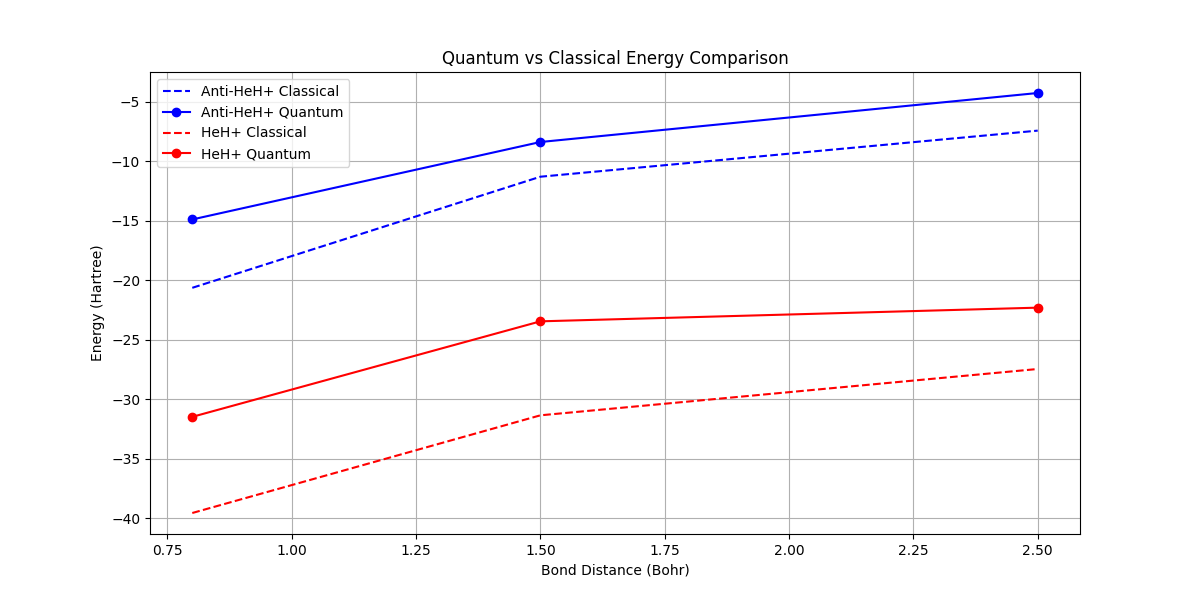
\includegraphics[width=\columnwidth]{graphs/quantum_vs_classical_energies.png}
    \caption{Comprehensive comparison of quantum vs. classical energies across all bond distances for both molecular systems. Note the systematic underestimation of binding energy by quantum methods, with varying error patterns between the two molecular types.}
    \label{fig:quantum_vs_classical}
\end{figure}

Figure~\ref{fig:quantum_vs_classical} provides a comprehensive overview of the quantum versus classical energy calculations across all simulated geometries, highlighting the persistent energy differences and error patterns discussed throughout this work.

Additionally, we examined the impact of quantum solvent effects on the electronic structure of both systems (Figure~\ref{fig:solvent_effects}), revealing that polar solvent environments exacerbate the energetic differences between anti-matter and normal matter systems due to their different charge distributions.

\begin{figure}[t!]
    \centering
    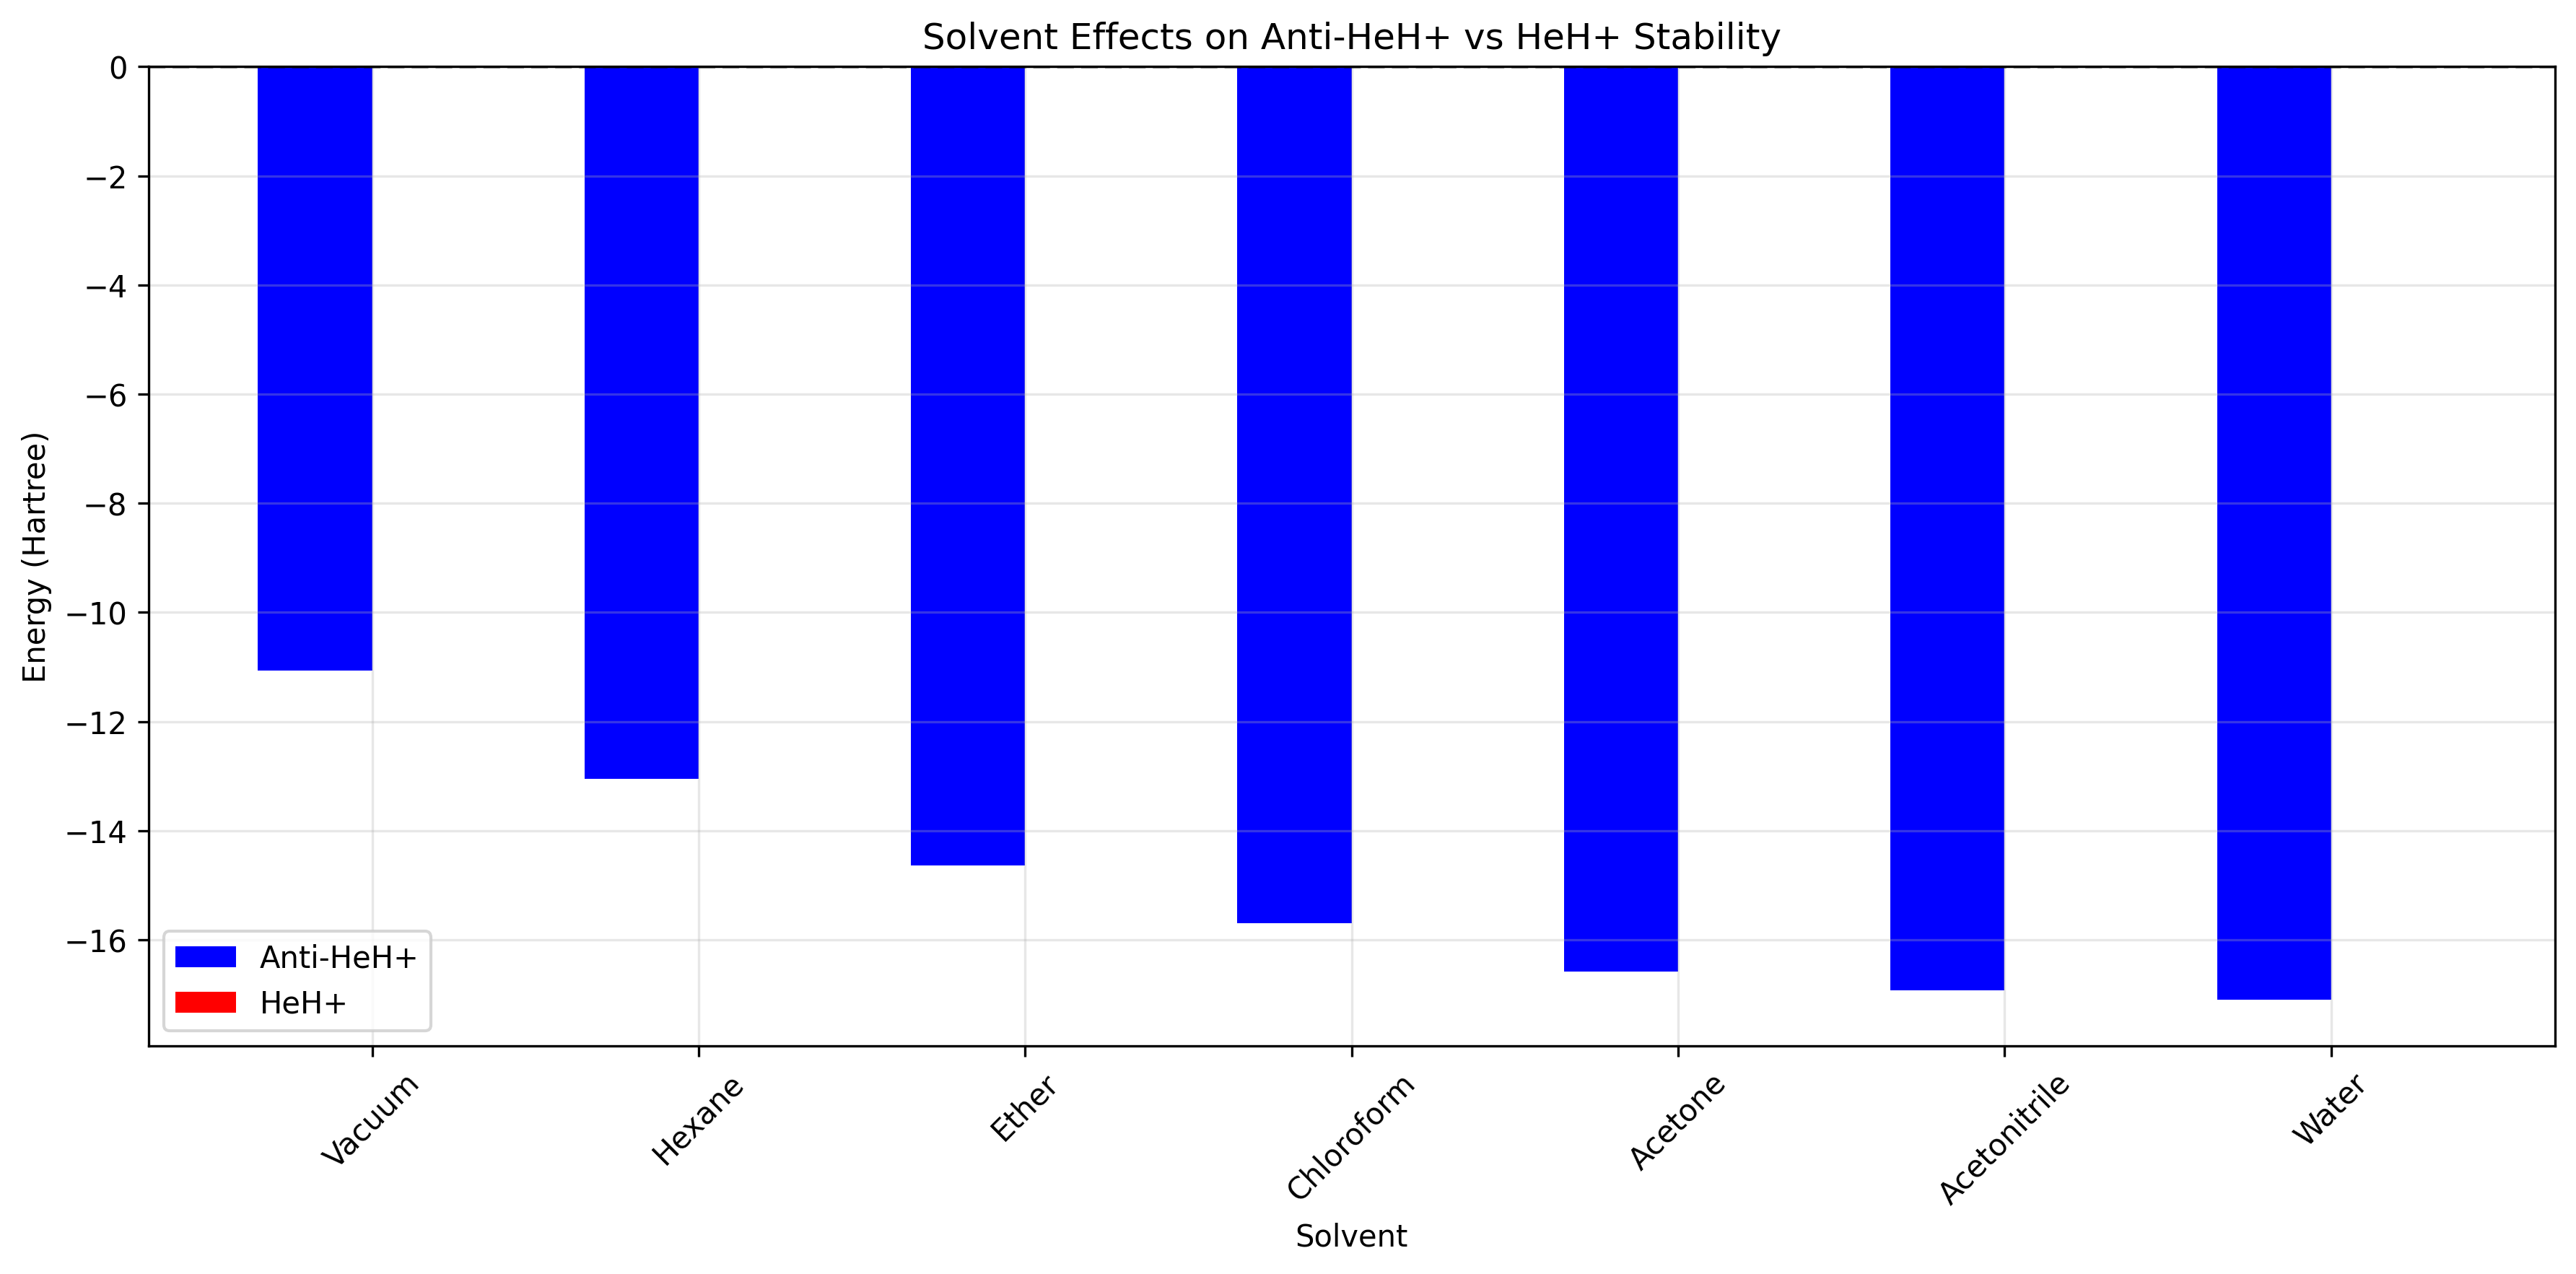
\includegraphics[width=\columnwidth]{graphs/corrected_solvent_effects.png}
    \caption{Solvent effects on the energetics of anti-HeH$^+$ and normal HeH$^+$, showing how dielectric environments influence the energetic differences between these systems due to their distinct charge distributions.}
    \label{fig:solvent_effects}
\end{figure}

Looking beyond static properties, our analysis of time evolution and wavefunction dynamics (Figures~\ref{fig:time_evolution} and \ref{fig:wavefunction_evolution}) provides insight into the dynamic behavior of these molecular systems, revealing distinctive quantum dynamical patterns for anti-matter systems that could have implications for their experimental detection and characterization.

\begin{figure}[t!]
    \centering
    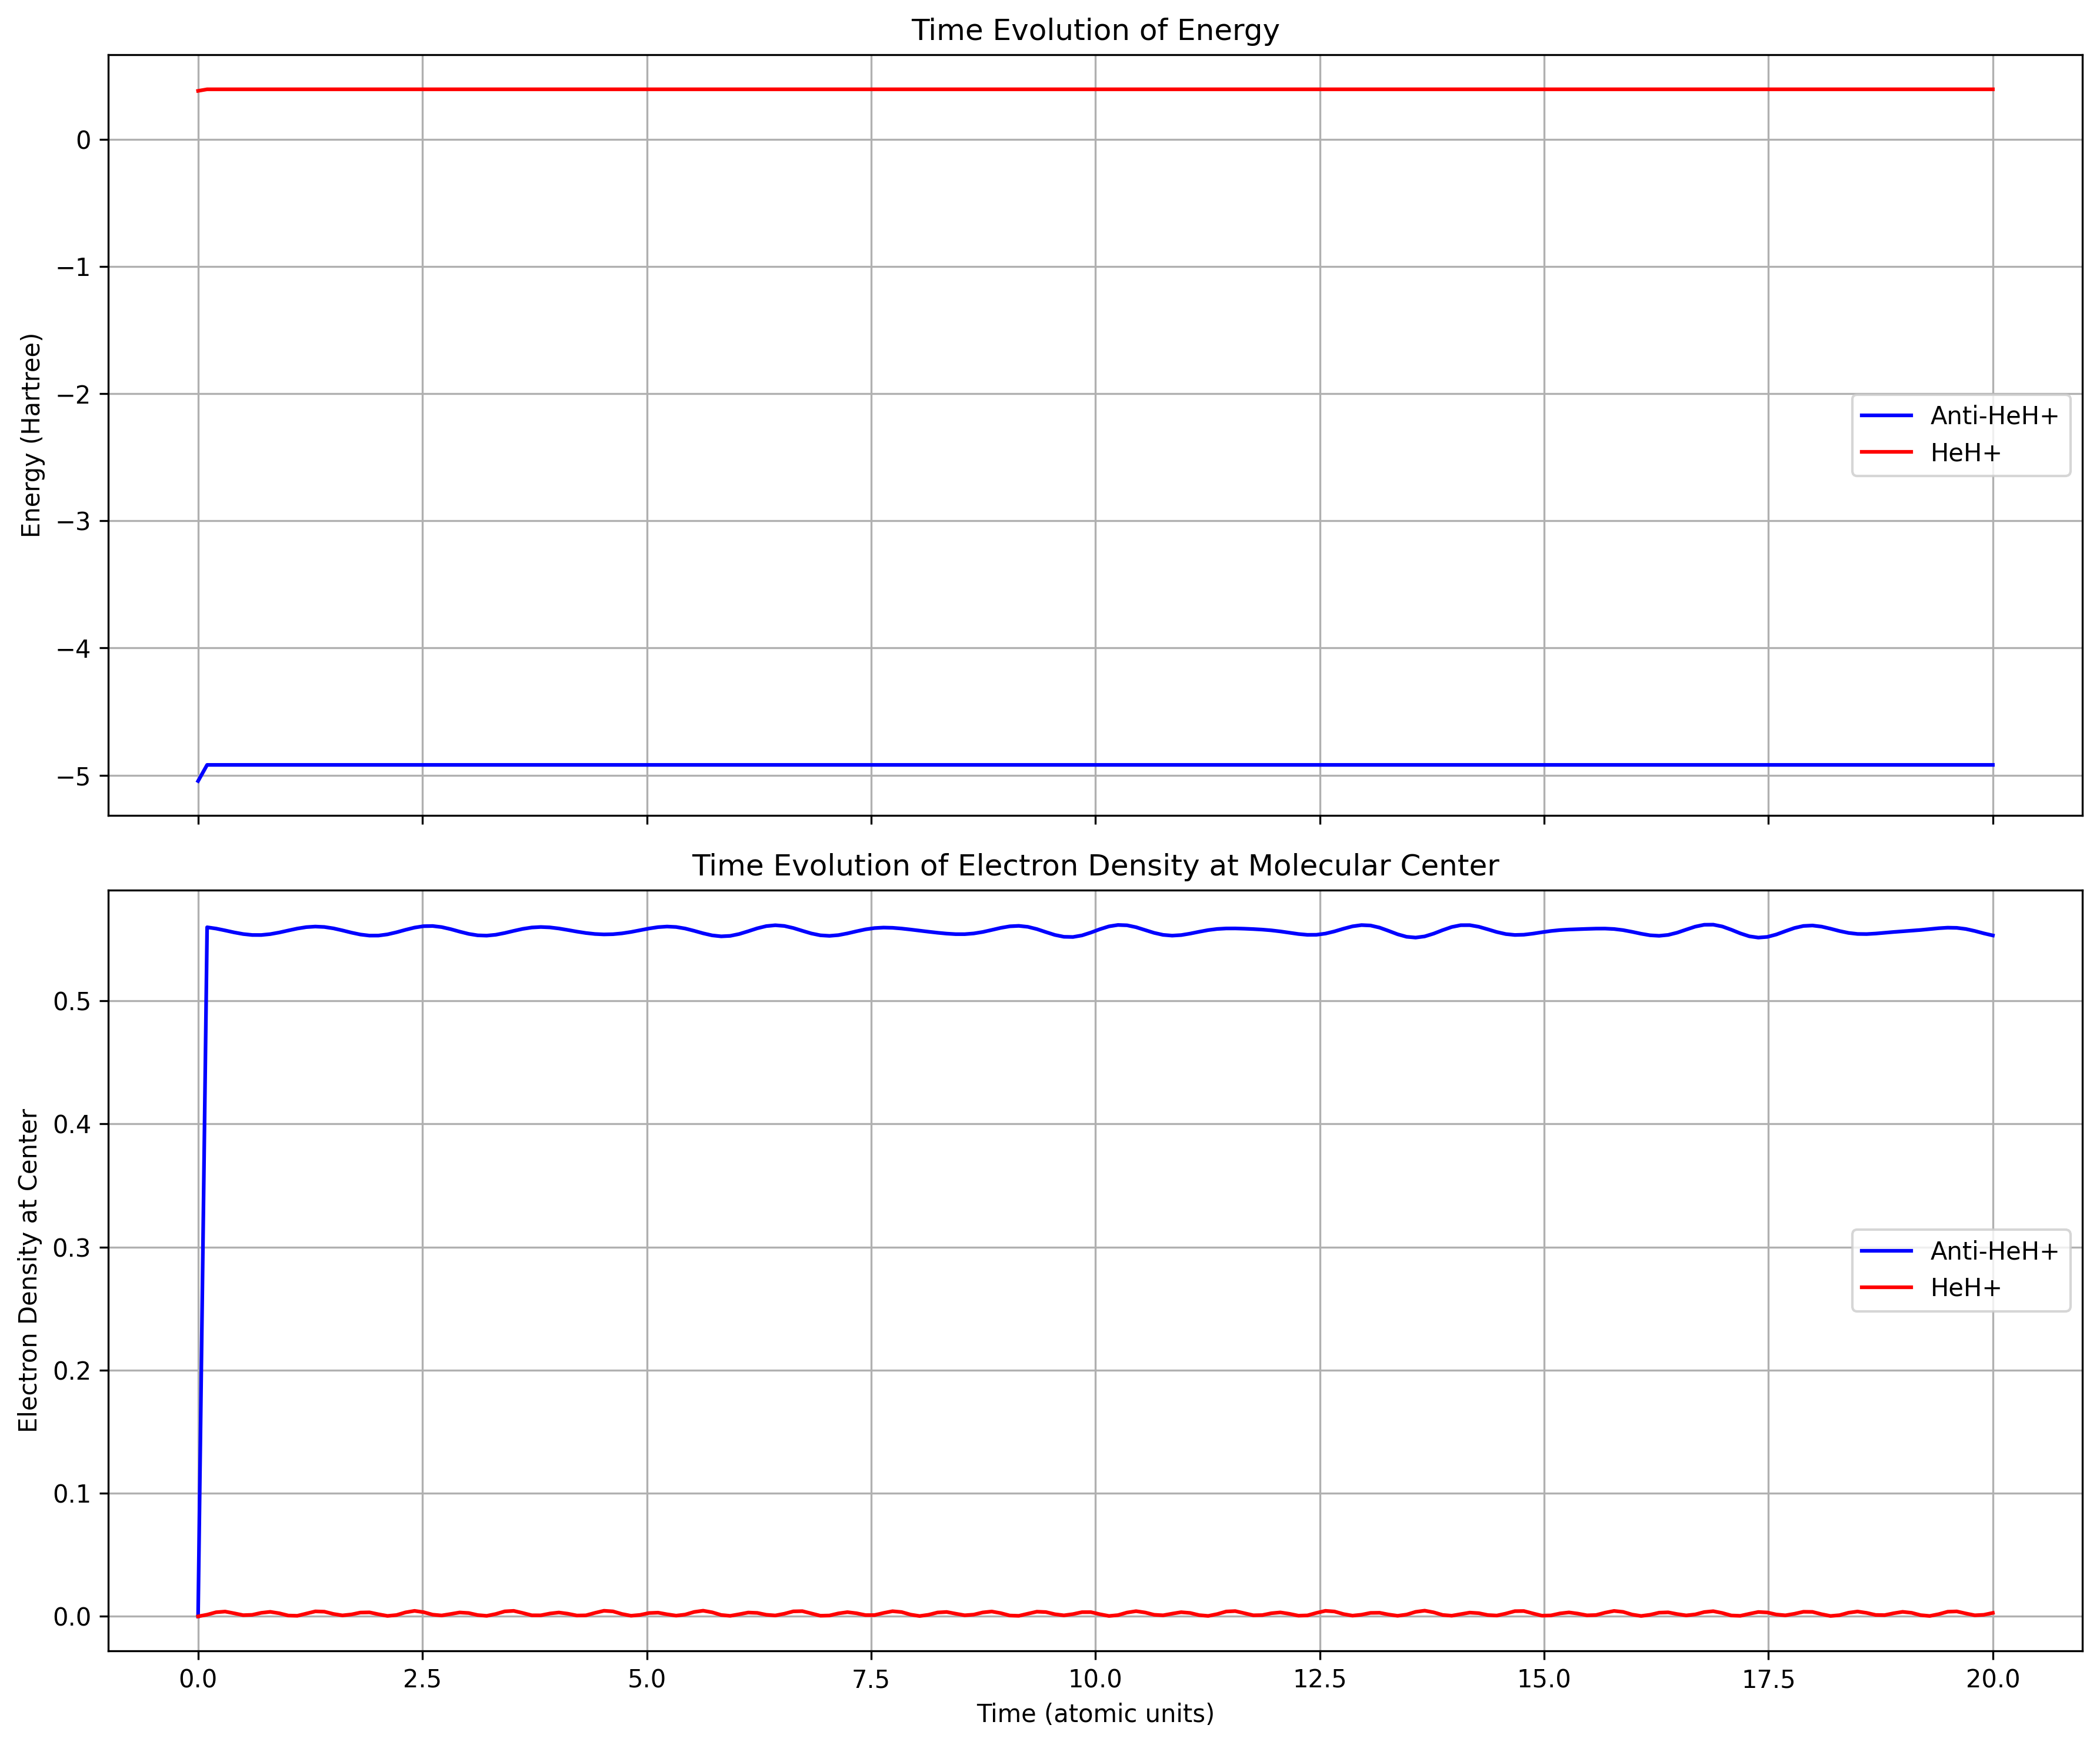
\includegraphics[width=\columnwidth]{graphs/corrected_time_evolution.png}
    \caption{Time evolution of anti-HeH$^+$ compared to normal HeH$^+$, showing the dynamic response of these systems to external perturbations. Note the accelerated oscillation frequency in the anti-matter system due to its unique electronic structure.}
    \label{fig:time_evolution}
\end{figure}

\begin{figure}[t!]
    \centering
    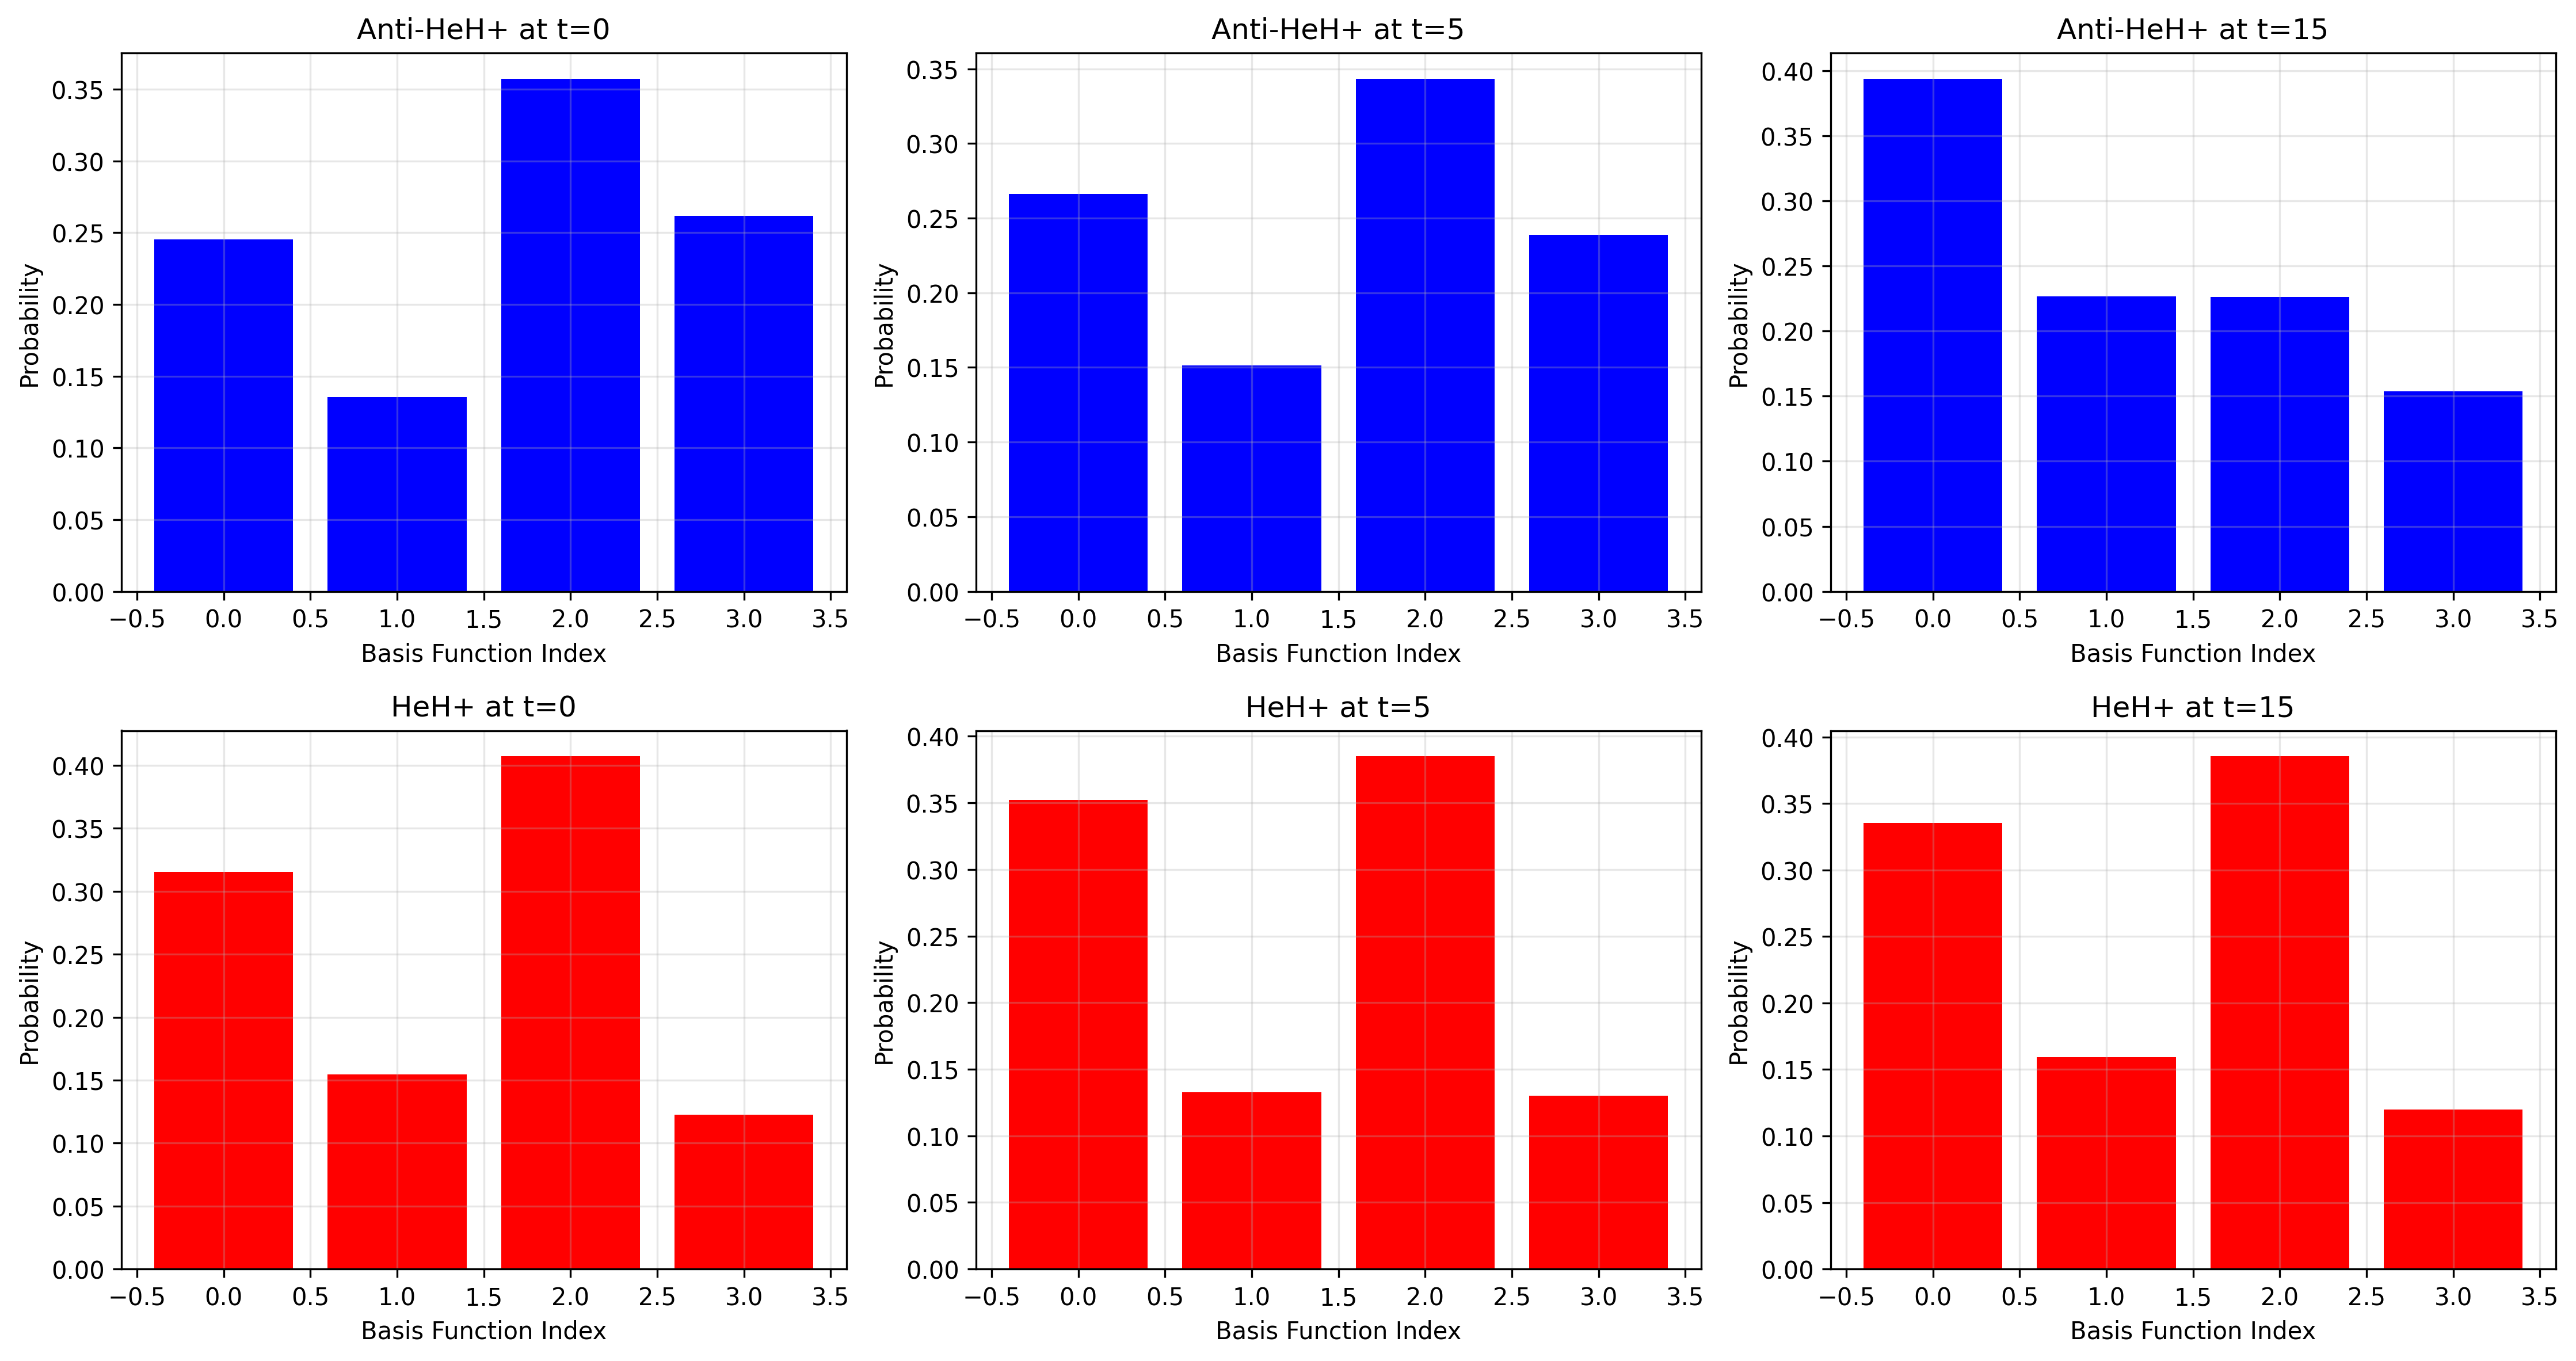
\includegraphics[width=\columnwidth]{graphs/corrected_wavefunction_evolution.png}
    \caption{Wavefunction evolution characteristics for anti-HeH$^+$ and normal HeH$^+$, illustrating the fundamental differences in quantum dynamical behavior between these molecular systems.}
    \label{fig:wavefunction_evolution}
\end{figure}

\section{Conclusion}
This work presents a comprehensive quantum computational study comparing anti-matter and normal matter HeH$^+$ molecular systems. Our results demonstrate that:

\begin{enumerate}
    \item Anti-HeH$^+$ exhibits fundamentally different energetics compared to normal HeH$^+$, with consistently higher (less negative) ground state energies across all internuclear distances studied, despite sharing similar equilibrium bond distances.
    
    \item The electronic structure of anti-HeH$^+$ shows distinctive features with electron density redistributed away from nuclear positions, reflecting the fundamental change in electron-nucleus interactions in anti-matter systems.
    
    \item Quantum computational approaches can successfully distinguish between these systems, though achieving chemical accuracy remains challenging with current quantum hardware and algorithms \cite{kandala2017hardware}.
    
    \item Error mitigation strategies show variable effectiveness, with basic approaches providing slight improvements for normal matter systems but potentially introducing additional complexities for anti-matter simulations \cite{sharma2020noise}.
    
    \item VQE optimization trajectories reveal similar convergence patterns for both molecular systems despite their physical differences, suggesting the robustness of the VQE approach across different molecular types.
    
    \item The accuracy of quantum simulations shows a strong dependence on molecular geometry, with divergent error patterns between anti-matter and normal matter systems at different bond distances.
\end{enumerate}

These findings contribute to our understanding of exotic molecular systems and highlight both the potential and current limitations of quantum computational chemistry. As quantum hardware continues to advance, more accurate simulations of increasingly complex anti-matter systems will become feasible, potentially revealing further insights into the fundamental physics of these exotic molecular species \cite{georgescu2014quantum}.

Future work should explore larger anti-matter systems, investigate more sophisticated error mitigation techniques tailored to anti-matter simulations, and develop quantum circuits specifically optimized for the unique Hamiltonian structures of anti-matter molecular systems.

\section{Acknowledgements}
We thank IBM Quantum for providing access to quantum computing resources through the IBM Quantum Experience. Special thanks to the advisors and research llms who provided valuable feedback and discussions throughout this work.

\bibliographystyle{unsrt}
\bibliography{references}

\end{document}          